\documentclass[11pt,a4paper,twoside,openright]{report}

\usepackage[dvips]{graphicx}
\usepackage{tabularx}
\usepackage{afterpage}
\usepackage{amsmath,amssymb}
\usepackage{bm}
\usepackage{mathtools}
\usepackage{rotating}
\usepackage{fancyhdr}
\usepackage{lipsum}
\usepackage[scriptsize]{caption}
% \usepackage{subcaption}
% \usepackage{algpseudocode}
\usepackage{algorithm}
\usepackage{subfig}
% \usepackage{tikz}
% \usepackage{pgfplots}
% \usepgfplotslibrary{fillbetween}
% \pgfplotsset{compat=1.14}
% \allowdisplaybreaks
\usepackage{algorithmic}
\usepackage{hyperref}
\usepackage[space]{grffile} % to use space in the file path
\usepackage{color}
\usepackage[usenames,dvipsnames]{pstricks}
\usepackage{epsfig}
\usepackage[usenames,dvipsnames]{pstricks}
\usepackage{epsfig}
\usepackage{pst-grad} % For gradients
\usepackage{pst-plot} % For axes
\usepackage[space]{grffile} % For spaces in paths
\usepackage{etoolbox} % For spaces in paths
\makeatletter % For spaces in paths
\patchcmd\Gread@eps{\@inputcheck#1 }{\@inputcheck"#1"\relax}{}{}
\makeatother
% User Packages:
\usepackage{amssymb,amsthm,amsmath}
\usepackage{mathtext}
\usepackage{amsthm}
% \usepackage[algcompatible]{algpseudocode}

\usepackage{placeins}
% To ensure figure to be in the correct subsection
%\usepackage{placeins}
%
%\let\Oldsection\section
%\renewcommand{\section}{\FloatBarrier\Oldsection}
%
%\let\Oldsubsection\subsection
%\renewcommand{\subsection}{\FloatBarrier\Oldsubsection}
%
%\let\Oldsubsubsection\subsubsection
%\renewcommand{\subsubsection}{\FloatBarrier\Oldsubsubsection}
\hyphenation{con-fi-gu-ra-zio-ne}

\setlength{\oddsidemargin} {2. cm}
\setlength{\evensidemargin} {2. cm}
\addtolength{\oddsidemargin} {-0.4 cm}
\addtolength{\evensidemargin} {-0.4 cm}
\linespread{1.1}

\usepackage[english]{babel}
% \usepackage[latin1]{inputenc}
\renewcommand{\captionfont}{\normalfont \sffamily \itshape \small}
\captionsetup[algorithm]{justification = raggedright, singlelinecheck = false}

\pagestyle{empty}

\newtheorem{definition}{Definition}[section]
\newtheorem{theorem}{Theorem}[section]
\newtheorem{corollary}{Corollary}[section]
\newtheorem{assumption}{Assumption}
\newtheorem{lemma}{Lemma}[section]
\usepackage[draft]{todonotes}
\DeclareMathOperator*{\argmin}{arg\,min}
\DeclareMathOperator*{\arginf}{arg\,inf}

\begin{document}
\thispagestyle{empty}
\vspace*{-1.5cm}
 \bfseries{
\begin{center}
  \large
  POLITECNICO DI MILANO\\
  \normalsize
  Mathematical Engineering Master Degree\\
  Dipartimento di Matematica\\
  \begin{figure}[htbp]
    \begin{center}
      \includegraphics[width=5cm]{./img/logo/Logo_Politecnico_Milano.png}
      % \includegraphics[width=5cm]{./img/logo/digi3.png}
    \end{center}
  \end{figure}
  \vspace*{0.1cm} \LARGE


    \textbf{Online Gradient Descent for Online Portfolio Optimization with Transaction Costs}\\


  \vspace*{.75truecm} \large
 %  \vspace*{0.5truecm} \large
  Artificial Intelligence and Robotic Laboratory \newline of Politecnico di Milano
\end{center}
\vspace*{2.0cm} \large
%\vspace*{2.0cm} \large
\begin{flushleft}


  Supervisor: Prof. Marcello Restelli \\

  \begin{tabbing}  
      Co-supervisors: \=  Francesco Trov\a`{o} Ph.D.,
      Edoardo Vittori,
  \end{tabbing}
\end{flushleft}
\vspace*{1.0cm}
%\vspace*{0.5cm}
\begin{flushright}


  Master thesis of:\\ Martino Bernasconi de Luca, 10465492\\


\end{flushright}
\vspace*{0.8cm}
\begin{center}

  Academic Year 2018-2019 % check
\end{center} \clearpage
}

\thispagestyle{empty} \normalfont \cleardoublepage
\thispagestyle{empty}  \cleardoublepage
\pagenumbering{Roman}
\begin{abstract}
Outperforming the markets through active investment strategies is one of the main challenges in finance.
The random movements of assets and the unpredictability of catalysts make it hard to perform better than the average market, therefore, in such a competitive environment, the methods designed to keep low transaction costs have a significant impact on the obtained wealth.
This thesis focuses on investing techniques to beat market returns through Online Portfolio Optimization while controlling transaction costs.
Such a framework differs from classical approaches as it assumes that the market has an adversarial behavior and no statistical characterization is assumed, requiring frequent rebalancing of the portfolio.
Within this context, most of the existing algorithms neglect transaction costs; we show that the one which provides bounded costs make unrealistic assumptions.
To deal with transaction costs, in the Online Portfolio Optimization setting, we propose the use of the Online Gradient Descent algorithm. We show that it has regret, considering costs, of the order $\mathcal{O}(\sqrt{T})$, $T$ being the investment horizon, and has $\Theta(N)$ per-step computational complexity, $N$ being the number of assets.
Furthermore, we show that this algorithm provides competitive gains when compared empirically with state-of-the-art online learning algorithms on real-world datasets.
\end{abstract}
\begin{poliabstract}{Sommario}
Una delle sfide più importanti in finanza è quella di avere prestazioni migliori rispetto ad un approccio passivo agli investimenti. I movimenti casuali del mercato e la difficoltà nel predirne i catalizzatori rendono molto complesso battere il mercato, e quindi, in un ambito tanto competitivo, tecniche progettate per tenere bassi i costi di transazione possono avere un impatto significativo sul guadagno finale. Questa tesi si concentra su tecniche di investimento basate su \emph{Online Portfolio Optimization} controllando i costi di transazione. Questo ambito si differenzia dal classico approccio poiché assume che i mercati abbiano un comportamento avversario, ossia non richiede delle assunzioni sul modello stocastico del processo, il che richiede quindi che tali tecniche ridistribuiscano di frequente il loro portfolio. Molti degli algoritmi in questo ambito non considerano i costi di transazione; mostreremo che quelli che hanno delle garanzie teoriche sui costi lo fanno con assunzioni irrealistiche. Si propone l'uso di \emph{Online Gradient Descent} per trattare il problema dei costi di transazione in Online Portfolio Optimization. Mostreremo che questo algoritmo assicura un regret sul guadagno con costi dell'ordine di $\mathcal O(\sqrt T)$, dove $T$ è l'orizzonte temporale. Inoltre mostreremo che questo algoritmo ha complessità computazionale dell'ordine di $\Theta(N)$, dove $N$ è il numero di azioni nel portfolio.
Infine verificheremo sperimentalmente le garanzie teoriche dell'algoritmo e che esso, quando testato su dati reali, provvede a guadagni comparabili agli altri algoritmi nello stato dell'arte. Abbiamo testato gli algoritmi scelti su tre datasets usati comunemente in letteratura e su un dataset raccolto per questo lavoro. Su tutti i dataset otteniamo guadagni medi del portfolio comparabili agli altri algoritmi per piccoli valori del tasso di transazione (guadagno annualizzato di tra 8\% e 15\%, approssimativamente), e guadagni più grandi, rispetto agli altri algoritmi, per quasi tutti i dataset utilizzati. 

\end{poliabstract}
%\thispagestyle{empty} \vspace*{.75truecm} \cleardoublepage
%\include{chapters/acknowledgements}
\thispagestyle{empty} \vspace*{.75truecm} \normalfont \cleardoublepage
\pagestyle{plain}\renewcommand{\chaptermark}[1]{\markboth{\chaptername\ \thechapter.\ #1}{}}
\renewcommand{\sectionmark}[1]{\markright{\thesection.\ #1}}
\fancyhead[LE,RO]{\bfseries\thepage}
   
\fancyhead[RE]{\bfseries\leftmark} 
\fancyhead[LO]{\bfseries\rightmark}   
\renewcommand{\headrulewidth}{0.3pt}

\setcounter{tocdepth}{3}
\setcounter{secnumdepth}{3}
\tableofcontents

\listoffigures
% \listoftables
\listofalgorithms
\addtocontents{loa}{\def\string\figurename{Algorithm}}

\pagenumbering{arabic}
\chapter{Introduction}

Until the 50s, investing relied solely on the expertise of the managers. Afterwards, portfolio management became contaminated with ideas from economics, which at that time was already based on a rigorous mathematical formulation, stemming from statistics and probability.
This led to the birth of portfolio theory \cite{markowitz1952portfolio}. 
The problem of portfolio optimization is paramount as the amount of assets managed by funds and private investors is currently more than $85$ trillion USD, a quantity comparable to the global GDP.\footnote{\url{https://www.opalesque.com/671554/Global_assets_under_management_rose_to155.html}.}

Classical investment techniques for portfolio management assign a statistical distribution to the returns of the assets. Then, once the statistical model has been chosen, the problem is solved by optimizing the expected value of the utility of some random variable (usually accounting for the trade-off between risk and return) that describes the value of the portfolio in some fixed time point in the future. This line of thinking has been proposed and sustained by Markowitz, Samuelson and Fama \cite{markowitz1952portfolio}, and it is now called Modern Portfolio Theory (MPT). 

This approach is the standard in academia and when designing portfolios in practice, but it is known to be very susceptible to errors in the modeling of the random variables that model the asset returns. 
Indeed, it is known that markets have a non-stationary behavior, which means that any statistical assumption is ephemeral and unreliable \cite{schmitt2013non}. This techniques are also referred to as backward looking, \emph{i.e.}, they optimize w.r.t. inferences made on past realizations. In the complex financial environment of the past decades (and of present times) we saw how unpredictable certain events can be, and how any statistical assumption can be out-turned overnight.

In this thesis, we present an orthogonal and lesser-known approach of \emph{Online Portfolio Optimization} that originated from the fields of information theory at the Bell Labs in the 1950s, from the works of Shannon, Kelly and Cover. These methods were included in the classical portfolio theory framework, under the name of Capital Growth Theory \cite{hakansson1995capital}, \cite{maclean2011kelly}, and then got included in the machine learning literature under the framework of Online Learning \cite{cesa2006prediction}. Only recently this field has been taken into the Online Optimization field too \cite{hazan2016introduction}. This formulation of sequential decision making has interesting properties, such as stability in a game theory fashion (\emph{e.g.}, equilibrium) and robustness versus adversarial manipulation.
This approach has been successfully applied to gambling and sports betting \cite{thorp1966beat}, \cite{hausch1981efficiency}. The fascinating story of these works can be found in \cite{poundstone2010fortune}.

One of the most important points in favor of the techniques in Online Learning are the strong theoretical guarantees provided by algorithms developed under this framework. These guarantees come from the game theory concept of \emph{Regret}, which is a form of dissatisfaction originated from having taken an action, measured against the best actions taken by a class of  adversaries, called \emph{Experts}. The guarantees, that algorithms in this framework achieve, are of performing asymptotically as good as the best player in the expert class.

Principal in this thesis will be the extension of the theoretical framework of these methodologies to the presence of transaction costs in financial applications, and to provide strong theoretical assurance even in the presence of transaction costs. Indeed, in many financial situations transaction costs are not modeled and this can lead to over-optimistic findings. We think that research in this direction can eventually bridge the gap between practical applications and academic research in Online Portfolio Optimization.

To tackle this problem we propose the Online Gradient Descent algorithm for the Online Portfolio Optimization framework. Furthermore, we show that it has theoretical guarantees on the wealth and on the transaction costs in which it incurs during the investment period. Finally we present an experimental campaign to show that our proposed algorithm has good empirical performances on the wealth obtained in the absence of trading costs, and w.r.t. the transaction cost rate.

\section{Structure of the Thesis}

In Chapter \ref{ch:OnlineLearning} we present the classical framework of Online Learning, starting from the framework of Online Learning with Expert Advice. We then draw the connections with more classical frameworks of Game Theory and present the Online Convex Optimization framework, which is the most suited to embed the problem of Online Portfolio Optimization. 

In Chapter \ref{ch:OPO} we introduce the problem of probability assignment and how this is a natural extension of the Prediction with Experts advice presented in Chapter \ref{ch:OnlineLearning}. We then draw the connections of the problem of probability assignment to information theory, where the field of Online Portfolio Optimization was originally developed. The main reason of Chapter \ref{ch:OnlineLearning} and \ref{ch:OPO} is to introduce the theory necessary to understand the algorithms used in the Online Portfolio Optimization.

From Chapter \ref{ch:transaction_costs} onwards, we will formally present our extended framework of Online Portfolio Optimization with Transaction Costs, and introduce the central concept of Total Regret, that we will use in throughout the thesis. In Chapter \ref{ch:algos} we will present the algorithms of  state of the art of the Online Portfolio Optimization framework, and explain their connections to the theoretical framework presented in Chapter \ref{ch:OnlineLearning} and \ref{ch:OPO}. In Chapter \ref{ch:OGD} we will extend the celebrated Online Gradient Descent algorithm to the Online Portfolio Optimization with Transaction Costs, and prove its theoretical guarantees in this framework.

In Chapter \ref{ch:experiments} we present the numerical results of the Online Portfolio Optimization with Transaction Costs problem,on a variety of different datasets. Finally, Chapter \ref{ch:conclusions} summarizes the main contributions of this work, and details the possible future developments.

\pagenumbering{arabic}
\chapter{Online Learning}\label{ch:OnlineLearning}
Online Learning is a theoretical framework to formalize a sequential decision problem in which an agent has to take consecutive actions in an environment. Every time the agent takes an action, the environment returns a loss signal (or reward depending on the convention on the sign). This framework is similar to other sequential decision problems such as Reinforcement Learning \cite{sutton1998introduction}, with the main difference that the loss function is decided by an adversary which has complete knowledge of your strategy in advance, rather that be described by a stochastic probability kernel. \todo{F: è sbagliato.}
The purpose of this section is to present the general framework of Online Game Playing and to introduce the notation necessary for the development of the theory for Online Portfolio Optimization. We will define formally the framework of Online Learning with Expert Advice, which is one the most studied framework of Online Learning, due to its ability to include many other frameworks, such as Multi Armed Bandit \cite{bubeck2012regret} or Online Convex Optimization \cite{hazan2016introduction}.
Then we will present the concept of \emph{regret} and present the relationship of Online Learning to classical repeated games, a classical framework coming from the field of Game Theory. 
We are interested in this framework in order to model repeated investments in this framework. 
Modern finance \todo{F: direi anche che ci immaginiamo che esitanto degli avversari che possono giocare strategicamente... M: non pensavo fosse un concern i veri avversari.} has more and more the need for a Game Theoretic approach, this is evident when one looks at the field of \emph{On venue Market Making}, that can be modeled naturally as a repeated game, or in merger and acquisition that can be modeled as a normal form game \cite{Yanqing_MaA}. 
Finally we will introduce Online Convex Optimization as a special case of Online Learning with expert advice and its interesting relationship to theoretical statistical learning. The choice of this path, from Online Learning to Online Convex Optimization, has been done to show how general and powerful Online Learning is in its simplicity, and why Online Convex Optimization is the most suitable framework to present our contribution to Online Portfolio Selection, a framework that will be presented in Chapter \ref{ch:OPO}.

In fact, even if we will focus on the portfolio problem, the apparently simple formulation of this framework is capable to encompass many other applications and problems, such as network routing~\cite{belmega2018online} and dark pool order allocation~\cite{agarwal2010optimal}. 
A thorough dissertation of the techniques that have been developed in the field of Online Learning can be found in \cite{cesa2006prediction}.
%Cita qualcuno he dia esposizione completa

\section{Online Learning}
\label{sec:OnlineLearning}
\begin{definition}(Online Game Playing).\label{def:OGP}
    Let $\mathcal Y$ be the outcome space, $\mathcal D$ the prediction space and $f:\mathcal D\times\mathcal Y\to \mathbb R$ is a loss function, an Online Game is the following sequential game played by the forecaster $\mathcal A$ and the environment:

    For each round $t\in \mathbb N$
    \begin{enumerate}
        %\item Each expert $E_i\in\mathcal E$ choose its prediction $x_{t,E_i}\in\mathcal D$
        \item The learner $\mathcal A$ chooses an element of the decision space $x_t\in\mathcal D$.
        \item The environment chooses the element $y_t\in\mathcal Y$, and subsequently determines the loss function $f(\cdot,y_t)$.
        \item The agent $\mathcal A$ incurs in a loss $f(x_t,y_t)$.
		\item The agent updates its cumulative losses $L_t=L_{t-1}+f(x_t,y_t)$ with $L_0=0$.
    \end{enumerate}
\end{definition}\todo{F: algorithm}

In Online Learning an agent $\mathcal A$ has to guess the outcome $y_t$ based on the past sequence $y_1,y_2,\ldots,y_{t-1}$ of events that are in the outcome space $\mathcal Y$, at each time step the agent will play (sometimes we will also say \emph{predict}) $x_t$, that is an element of the prediction space $\mathcal D$, and the environment will choose a loss function $f(\cdot,y_t)$ by determining the outcome $y_t$.
The agent $\mathcal A$ is essentially the identification of the functions that map the history of past outcomes to the new prediction:
$$\mathcal A\equiv\left\{h_{t-1}:=(y_1,\ldots,y_{t-1})\longmapsto x_t\right\}_{t\ge 1}. $$
The simplest case is for $\mathcal Y=\mathcal D$ and both of finite cardinality, meaning that there are only a finite number of actions that the agent $\mathcal A$ can choose from. 
We will sometimes refer to the environment defined in Section \ref{def:OGP} as ``adversarial'', since no stochastic characterization is given to the outcome sequence $y_t$ and the analysis of the regret is done assuming a worst case scenario.
Since the adversary knows the prediction $x_t$, before deciding the outcome $y_t$, designing an algorithm which tries to minimize the loss is a hopeless task and so we have to set an easier scope. In Section \ref{sec:regret_and_experts} we will also present the counterexample to why the absolute minimization of the loss is an hopeless task, and present the adapt minimal framework to successful Online Learning in Adversarial Environment.

% ==================================================

% The assumption\todo{Non qui} of a model for the data even existing is basically assuming the stationarity of the observed events. This may be reasonable in some cases, like speech recognition in which we can assume that there is constant model which translate sound of speech into its lexical transliteration, but it not as reasonable in other cases, as trivial as spam filtering. In email classification for spam filtering, the spam writers actually adapts to the filter itself and every constant model would eventually be out of fashion after some time. In such a regime you need a way of adapting your hypotheses during the learning procedure. This is were Online Learning comes to help. In Online Learning we do not make any assumption on the structure of the data and constantly adapting our hypothesis in order to asymptotically perform as the best hypothesis in hindsight.

% =================================================

\subsection{Regret and Experts}\label{sec:regret_and_experts}
\begin{figure}[!ht]
\centering
\begin{pspicture}(0,-3.42)(8.18,3.42)
\psframe[linecolor=black, linewidth=0.04, dimen=outer, framearc=0.1](6.54,0.9)(2.78,-0.36)
\psframe[linecolor=black, linewidth=0.04, dimen=outer, framearc=0.1](6.52,3.42)(2.82,2.3)
\rput[bl](3.76,2.7){Agent: $\mathcal A$}
\rput[bl](3.68,0.12){Environment}
\psline[linecolor=black, linewidth=0.036, arrowsize=0.05291667cm 2.0,arrowlength=1.4,arrowinset=0.0]{->}(6.54,2.8)(7.66,2.8)(7.66,0.2)(6.54,0.22)
\rput[bl](7.9,1.44){$x_t$}
\psline[linecolor=black, linewidth=0.036, arrowsize=0.05291667cm 2.0,arrowlength=1.4,arrowinset=0.0]{->}(2.78,0.3)(1.46,0.3)(1.46,2.88)(2.8267796,2.8677726)
\rput[bl](0.0,1.2){$f(x_t,y_t)$}
\psframe[linecolor=black, linewidth=0.036, dimen=outer, framearc=0.1](6.2,-2.2)(3.16,-3.42)
\rput[bl](3.78,-2.92){Experts: $\mathcal E$}
\rput[bl](2.96,-1.36){$x_{e,t}$}
\rput[bl](5.26,-1.34){$f(x_{e,t},y_t)$}
\psline[linecolor=black, linewidth=0.036, arrowsize=0.05291667cm 2.0,arrowlength=1.4,arrowinset=0.0]{->}(3.8,-2.22)(3.8,-0.36)
\psline[linecolor=black, linewidth=0.036, arrowsize=0.05291667cm 2.0,arrowlength=1.4,arrowinset=0.0]{->}(5.18,-0.4)(5.18,-2.22)
\end{pspicture}

\caption{Online Learning with Expert Advice as Multi Agent-Environment interaction.}
\label{fig:OL}
\end{figure}

We stated that the objective of absolute loss minimization is hopeless in an adversarial framework, as the adversary can always choose the outcome $y_t$ that maximizes the loss $f(x,y_t)$ regardless of the decision $x\in\mathcal D$ taken by the learner. More formally, assume $\mathcal D$ to be the space of binary outcomes, \emph{i.e.} $|\mathcal D|=2$, and that $f$ is the absolute loss $f(x,y)=|x - y|$. Since the adversary plays after the learner $\mathcal A$, it can  make the loss of the learner $L_T=T$ by choosing $y=1-x$ as outcome the bit non predicted by the learner, making $f(x,y)=1$ at each time step. Notice that no assumption has been made on the strategy followed by the learner $\mathcal A$.
From this example it is clear that the learner has to set a less ambitious goal.

We do so by extending the theoretical formulation in Section \ref{sec:OnlineLearning} by including a set $\mathcal E$ of other players, this setting is called \emph{prediction with expert advice}. At each time step of the prediction game, each expert $e\in\mathcal E$, predicts an element $x_{e,t}\in\mathcal D$, and incurs in a loss $f(x_{e,t},y_t)$, just as the agent $\mathcal A$, creating a general multi-agent interaction as in Figure~\ref{fig:OL}. 
The goal of the learner is to obtain small losses with respect to the best expert in the class $\mathcal E$. This concept is captured by the definition of regret.
Formally, we define the regret $R_{e,T}$ for the agent $\mathcal A$ with respect to expert $e\in\mathcal E$ (assumed finite for the moment) as follows:

\begin{equation}\label{def:Regret}
	R_{e,T} = L_T-L_{e,T}.
\end{equation}

The regret observed by the agent $\mathcal A$ with respect to the entire class of experts $\mathcal E$ is defined as:

\begin{equation}
	R_T=\sup\limits_{e\in\mathcal E}R_{e,T}=L_T-\inf\limits_{e\in\mathcal E}L_{e,T}.
\end{equation}

The task agent $\mathcal A$ is to find a sequence $x_t$, function of the information obtained up to the time $t$ in order to obtain small regret $y_T$ with respect to any sequence $y_1,y_2,\ldots$ chosen by the environment.

In particular we aim to achieve sub-linear regret $R_T= o(T)$, meaning that the per-round regret $R_T/T$ will asymptotically vanish: 

\begin{equation}
	R_T= o(T) \implies \lim\limits_{T\to \infty}\frac{R_T}{T}=0,
\end{equation}

where $ o(T)$ is the space of sub-linear affine functions. A strategy $\mathcal A$ that attains sub-linear regret is called \emph{Hannan-Consistent}~\cite{hannan1957approximation}.

The regret is a measure of the distance between our online performance and the best offline (in retrospect) performance among the expert class $\mathcal E$, this is also called \emph{external regret} since it is compared to the external set of experts $\mathcal E$. A surprising fact is even that such algorithms do even exist.
Indeed a first result is that \emph{in general} there are no Hannan-consistent strategies, and just introducing the concept of regret is not enough by itself for successful Online Learning. 

A first simple counterexample can be found in~\cite{cover1966behavior}. If the decision space $\mathcal D$ is finite then there exists a sequence of loss function such that $R_T=\Omega(T)$.
% Cover Impossibility
Again take $\mathcal D$ as a space of binary outcomes, absolute loss as $f(x,y)=|x - y|$, and the class of experts is composed by two experts, one predicting always $0$ and the other always $1$. Taking $T$ odd, we have that the loss of the best expert is $L_{e,T}<\frac{T}{2}$, and we have already shown that the adversary can make the loss of the learner $L_T=T$. It is now evident that the regret is $R_T>T-\frac{T}{2}$, which does not allow $R_T/T\to 0$. This argument is easily extended in the case of any finite decision space $\mathcal D$.

To achieve sub-linear regret, the learner has to randomize its predictions, at each turn $t$, the agent choose a probability distribution on the decision space and plays $x_t$ according to this distribution. Clearly the adversary has knowledge of the probability distribution of the learner $\mathcal A$, but has no knowledge of the random seed used by the agent $\mathcal A$, \emph{i.e.} does not know the actual decision sampled from the distribution held by the agent. If the original decision space was $\mathcal D$ with $|\mathcal D|=N$ after the randomization of the decision, we effectively transformed the decision space $\mathcal D$ into the $\Delta_{N-1}\in\mathbb R^{N}$ probability simplex. By doing so we are formally extending the game into its mixed extension, as will be discussed further in Section \ref{sec:GT}. It can be viewed also as a \emph{covexification} of the domain, pointing to the undeniably necessity of convex geometry in this context, that will be discussed in Section \ref{sec:OCO}. Therefore, from now on the domain $\mathcal D$ will be convex, either by the problem specification or by randomized convexification if the problem has discrete decision space.

\subsection{Existence of No-Regret Strategies}\label{sec:existence_of_no_regret}
In this section we will show the existence of Hannan-consistent strategies in the case of finite experts and provide a general form to generate sub-linear regret strategies. 
The general idea with a finite class of experts is given by the Weighted Average Forecaster, which implements a the natural idea of playing as the weighted average of the experts predictions:

\begin{definition}(Weighted Average Forecaster).\label{def:weighted_avg}
For a finite class of experts $\mathcal E=\{E_1,\ldots,E_N\}$, the weighted average prediction is defined as
\begin{equation}
	x_t = \frac{\sum\limits_{i=1}^{N}w_{i,t-1}x_{i,t}}{\sum\limits_{i=1}^{N}w_{i,t-1}},
\end{equation}
where $w_{i,t-1}>0$ and $x_{i,t}$ is the prediction of expert $E_i\in\mathcal E$ at round $t$. 
\end{definition}

Since $\mathcal D$ is convex we have that $x_t\in\mathcal D$.
Then it is natural to assume that the weights are a function of the cumulated regret suffered by the agent with respect to the experts, and also that the change in weight is proportional to the change in a potential function.
We can generalize the simple weighted average prediction in Equation \eqref{def:weighted_avg} in the following general form, introduced in~\cite{cesa2003potential}:

\begin{equation}\label{eq:potential_avg}
x_t = \frac{\sum\limits_{i=1}^{N}\partial_i \Phi(\mathbf R_{t-1}) x_{t,i}}{\sum\limits_{i=1}^{N}\partial_i \Phi(\mathbf R_{t-1}) },
\end{equation}

where $\Phi(\mathbf u)=\varphi\left(\sum\limits_{i=1}^N\phi(u_i)\right)$ is a function $\Phi:\mathbb R^N\to\mathbb R^+$ defined through two increasing functions $\phi,\varphi:\mathbb R\to\mathbb R^+$, $\varphi,\phi\in\mathcal C^2(\mathbb R)$ concave and convex, respectively and $\mathbf R_T=(R_{1,T},\ldots,R_{N,T})$.
By specializing the two functions $\varphi,\phi$ we can derive most of the algorithms for dealing with prediction under expert advice.
The reasons behind the general form of Equation \eqref{eq:potential_avg} and an extended discussion can be found in~\cite{hart2001general}, \cite{cesa2003potential} and \cite{blackwell1956analog}, but the general idea is that the form of Equation \eqref{eq:potential_avg} has the following property:

\begin{theorem}\cite{cesa2003potential}
	If $x_t$ is given by Equation~\eqref{eq:potential_avg} and the loss $f(\cdot,y)$ is convex in the first argument then the instantaneous weighted regret satisfies:  
	$$\sup\limits_{y_t\in\mathcal Y}\sum\limits_{i=1}^N[f(x_t,y_t)-f(x_{i,t},y_t)]\partial_i \Phi(\mathbf R_{t-1}) \le 0.$$
\end{theorem}

\begin{proof}
	By convexity of $f(\cdot,y_t)$ we have that 
\begin{align}\label{eq:blw_cond}
	f(x_t,y_t)\le\frac{\sum\limits_{i=1}^N\partial_i\Phi(\mathbf R_{t-1})f(x_{i,t},R_t)}{\sum\limits_{i=1}^N\partial_i\Phi(\mathbf R_{t-1})}, \forall y_t\in\mathcal Y.
\end{align}
And since $\Phi(\mathbf x)=\varphi\left(\sum\limits_{i=1}^N \phi(x_i)\right)$ we have that $$\partial_i\Phi(\mathbf x)=\varphi'\left(\sum\limits_{i=1}^N\phi(x_i)\right)\phi'(x_i)\ge0.$$
Hence we can rearrange the terms in Equation~\eqref{eq:blw_cond} to obtain the statement.
\end{proof}

Note that fixing the structure for the weights as in Equation \eqref{eq:potential_avg} we have that $w_{t,i}\propto\phi'(R_{i,t})$ is an increasing function in $R_{i,t}$ (since $\phi$ is convex and increasing) that essentially states that we are increasing the probability of playing actions on which we saw high regret $R_{i,t}$\todo{check!!!}.

\begin{definition}(Exponentially Weighted Algorithm)\label{def:ewf}
	The Exponentially weighted algorithm is obtained from Eqaution \eqref{def:weighted_avg} by defining:
	\begin{equation}\label{eq:weights_ewf}
	w_{i,t-1}=e^{\eta y_{i,t-1}}/\sum\limits_{j=1}^Ne^{\eta y_{j,t-1}}.
	\end{equation}
\end{definition}

Note that, the exponentially weighted algorithm is also Equation \eqref{eq:potential_avg} where we defined $\varphi(x)=\frac{1}{\eta}ln(x)$ and $\phi(x)=e^{\eta x}$ giving weights defined in Equation \eqref{eq:weights_ewf}.

It can be shown (\cite{cesa2006prediction} Theorem 2.2) that the algorithm defined by the update rule in Equation \eqref{def:ewf}, and for a convex loss function $f(\cdot,y_t)$, gives the following guarantee on the regret:
\begin{equation}\label{eq:regret_ewf}
R_T\le \frac{log(N)}{\eta}+\frac{T\eta}{8}.
\end{equation}

By choosing $\eta=O\left(\sqrt\frac{1}{T}\right)$ we obtain a sub-linear regret $R_T=\mathcal O(\sqrt T)$. %It is also possible to make this algorithm an all-time algorithm (no need to know the length of the game $T$, as opposed as a \emph{one-time} algorithm) by using the so called doubling trick by continually adapting the parameter $\eta$. In general a one-time algorithm obtains slightly smaller bounds then the all-time counterparts, that require the knowledge



\section{Experts}
The theoretical framework described in Section \ref{sec:OnlineLearning} is very general and most suited for a game theory analysis of the problem. This helps us describe many other frameworks, such as Online Optimization \cite{hazan2016introduction}, or Multi Armed Bandit \cite{bubeck2012regret} as embedded into a Game Playing framework with expert advice. It can then be specialized by fixing many elements of the definition, in order to be applied to the specific problem we are willing to solve.
For instance, the class of experts $\mathcal E$ is most of the time completely fictitious, meaning that the experts are not real players of the game, but most of the time they are \emph{simulable} meaning that the agent $\mathcal A$ is able to compute $x_{e,t}$ for each expert $e\in\mathcal E$ and most of the times the class of expert is very limited in its actions, \emph{e.g.}, $\mathcal E$ is the class of experts for which $x_{e,t}$ is constant in $t$. In this case, which is the most studied class of experts, we are basically just comparing our learner $\mathcal A$ to the best fixed action $x^*$ in hindsight. This is a clairvoyant strategy that attains the minimum cumulative loss over the entire length of the game $T$.

\subsection{Uncountable Experts}\label{sec:uncountable_exp}

In the case of uncountable experts the Exponentially Averaged Prediction cannot be applied directly, but can be extended to a continuous mixture of experts predictions. More specifically we need the case of the class $\mathcal E$ being generated by a convex hull of a finite number of a base class of experts, $\mathcal E_N$.
With continuous class of experts $\mathcal E$ defined in this way, the regret definition becomes:

\begin{equation}
    R_T = \sup\limits_{\mathbf q\in\Delta_{N-1}}R_{\mathbf q,T}:=L_T-\inf\limits_{\mathbf q\in\Delta_{N-1}}L_{\mathbf q,T},
\end{equation}

where $\Delta_{N-1}\subset \mathbb R^{N}$ is the $N$-simplex, and 

$$L_{\mathbf q,T}=\sum\limits_{t=1}^T f(\langle \mathbf q,\mathbf x_{e,t}\rangle,y_t),$$
where $\mathbf x_{e,t}=(x_{1,t},\ldots,x_{N,t})\in\mathbb R^N$ is the vector of expert predictions at time $t$.


\section{Exp-Concave loss functions}\label{sec:exp-concave-mixture}

Very important for the study of Portfolio Optimization is the exp-concave class of loss functions. The reason is that the natural loss function used in the Online Portfolio Optimization framework, is $1$ exp-concave, as we shall see in Chapter \ref{ch:OPO}.

\begin{definition}(Exp-concave function). 
$g(x)$ is said $\nu$ exp-concave if $e^{-\nu g(x)}$ is concave.
\end{definition}

When speaking about loss functions we are interested in concavity of the function in its first argument. Therefore we will say that a loss function $f$ is $\nu$ exp-concave if $f(\cdot,y)$ is $\nu$ exp-concave $\forall y\in\mathcal Y$. 

\begin{theorem}\label{th:General_Blk}(\cite{cesa2006prediction} Theorem 3.2)
The Exponentially Weighted Average forecaster, for $\nu$-exp concave loss functions has the following property taking $\eta=\nu$:

$$\Phi(\mathbf R_T)\le \Phi(\mathbf R_0),$$

where $\Phi(x)=\varphi\left(\sum\limits_{i=1}^N\phi(x_i)\right)$ is chosen as $\varphi(x)=\frac{1}{\nu}log(x)$ and $\phi(x)=e^{\nu x}.$

\end{theorem}

\begin{proof}
    The weights are given by $w_{i,t-1}=e^{\nu y_{i,t-1}}/\sum\limits_{j=1}^N e^{\nu y_{j,t-1}}$.
    By exp-concavity we have that
    \begin{equation}
        e^{-\nu f(x_t,y_t)}=exp\left\{-\nu f \left(\frac{\sum\limits_{i=1}^N w_{i,t-1}x_{i,t}}{\sum\limits_{i=1}^N w_{i,t-1}},y_t\right)\right\}\ge \frac{\sum\limits_{i=1}^N w_{i,t-1}e^{-\nu f(x_{i,t},y_t)}}{\sum\limits_{i=1}^N w_{i,t-1}}.
    \end{equation}
    This can be rewritten as 
    \begin{equation}\label{eq:conc_exp_last}
        \sum\limits_{i=1}^N e^{\nu y_{i,t-1}}e^{\nu [f(x_t,y_t)-f(x_{i,t},y_t)]}\le \sum\limits_{i=1}^N e^{\nu y_{i,t-1}}.
    \end{equation}
    Applying $\varphi(x)=\frac{1}{\nu}log(x)$ to both sides of Equation \eqref{eq:conc_exp_last} we obtain that $$\Phi(\mathbf R_{t})\le \Phi(\mathbf R_{t-1}),$$ that proves the thesis.
\end{proof}

The case of exp-concave functions is very special, since we can obtain Theorem~\ref{th:General_Blk} that can be used to prove regret bounds very easily as:

\begin{equation}\label{eq:regret_exp_finite}
    R_T\le \frac{1}{\eta}\log\left(\sum\limits_{i=1}^N e^{\nu R_{j,T}}\right)=\Phi(\mathbf R_T)\le\Phi(\mathbf R_0) = \frac{log N}{\eta}.
\end{equation}

The case of exp-concave losses is also useful for the case of uncountable experts sketched in Section~\ref{sec:uncountable_exp}. This formulation will be of central importance for the portfolio optimization problem.

It is natural to extend the Exponential Weighted Majority algorithm described by Equation \eqref{def:weighted_avg} into the case of uncountable expert class $\mathcal E$ generated by the convex hull over the countable class $\mathcal E_N$, by:

\begin{equation}\label{eq:mixture}
    x_t=\frac{\int\limits_{\Delta_{N-1}} w_{\mathbf q,t-1}\langle \mathbf q, \mathbf x_{e,t}\rangle d\mathbf q}{\int\limits_{\Delta_{N-1}} w_{\mathbf q,t-1}d\mathbf q}.
\end{equation}

\begin{theorem}(Mixture forecaster for exp-concave losses)\\
(\cite{cesa2006prediction} Theorem 3.3).\label{th:mixture_forecaster}\\
    Choosing $w_{\mathbf q,t-1}=exp\left\{-\nu\sum\limits_{s=1}^{t-1}f(\langle \mathbf q,\mathbf x_{e,t}\rangle,y_s)\right\}$ in Equation \eqref{eq:mixture}, for a bounded $\nu$-exp concave loss function $f(\cdot,y)$, we obtain
    $$R_T\le \frac{N}{\nu}\left(log\left(\frac{\nu T}{N}\right)+1\right).$$
\end{theorem}

Even in the case of uncountable many experts, exp-concavity of the loss function gives a better convergence rate of $\mathcal O(\log T)$ then the exponentially weighted algorithm in Equation~\eqref{eq:regret_ewf}, which is $\mathcal O(\sqrt T)$.

% REGRET MINIMIZATION IN GAMES =================================================
\section{Regret Minimization in Games}
\label{sec:GT}
In this section we explore the connection of the framework of Section \ref{sec:OnlineLearning} into a more classical repeated game framework. In the previous section we looked at the adversary as a black box, without any specific model in mind. The reason of this chapter is to clarify its role as a player in the game and to show the game theoretical properties of Hannan-consistent agents. Since in Online Learning the convention is to speak about losses, we shall speak about losses (players are minimizing) also in the classical definitions of game theory instead of payoffs (players are maximizing).

\begin{definition}(Strategic Form $K$-Player Game).\label{def:Game}
    A Strategic form $K$-player game is t a tuple $\langle\mathcal K,\{X_i\}_{i\in\mathcal K},\{l_i\}_{i\in\mathcal K}\rangle$ where
    \begin{enumerate}
        \item $\mathcal K=\{1,\ldots,K\}$ is the finite set of players.
        \item $X_i$ is the set of actions available to player $i\in\mathcal K$.
        \item $l_i:\bigotimes\limits_{k=1}^KX_i\to\mathbb R$ is the loss observed by player $i\in\mathcal K$.
    \end{enumerate}
	The game is called finite if $|X_i|<+\infty$ for all $i\in\mathcal K$.
\end{definition}


\subsection{Mixed extension}\label{sec:mixed}
In Section~\ref{sec:OnlineLearning} we saw that it is impossible to obtain sub-linear regret in adversarial environment with finite decision space $\mathcal D$. A first step to solve this has been the \emph{randomized convexification} technique, where finite action spaces are extended into convex sets, given by their probability simplex. Losses are to be interpreted as expected losses when the mixed extension is applied to the formal game. More formally: 

\begin{definition}(Mixed-extension for finite games).
A finite game $\langle\mathcal K,\{X_i\}_{i\in\mathcal K},\{l_i\}_{i\in\mathcal K}\rangle$ can be extended into the game $\langle\mathcal K,\{\tilde X_i\}_{i\in\mathcal K},\{\tilde l_i\}_{i\in\mathcal K}\rangle$
\begin{enumerate}
	\item $\tilde X_i=\Delta_{|X_i|-1}\subset \mathbb R^{|X_i|}$ for all $i\in\mathcal K$ 
	\item $\tilde l:\bigotimes \tilde X_i\to\mathbb R$ is defined as
	$$\tilde l(x_1,\ldots,x_K)=\sum\limits_{i_1=1}^N\cdots\sum\limits_{i_K=1}^Np_{i_1}\ldots p_{i_K}l(i_1,\ldots,i_K).$$ 
\end{enumerate}
\end{definition}

Due to the impossibility result of Cover~\cite{cover1966behavior}, we have to work with the mixed extension formulation of the game. So from now on we take this step implicitly.
The taxonomy of game definition is quite extended and complex, we will focus on non-cooperative games \cite{nash1951non} since they are closely related to the setting tacked in the Online Learing field. More specifically, we will need the model for \emph{Zero Sum Game}. 

\begin{definition}($2$-Player Zero-Sum Game).\label{def:ZSG}
A Zero Sum game is a tuple $\langle\{X_1,X_2\},l:X_1\times X_2\to\mathbb R\rangle$. As in Definition~\ref{def:Game} $X_1,X_2$ are the action spaces for Player $1$ (row player) and Player 2 (columns player) respectively and $l(x_1,x_2)$ for $x_i,x_2\in X_1\times X_2$, represents the losses for Player $1$ and profits for player $2$.
\end{definition}

If this game is played for $T$ turns, we can call it a repeated game, and the losses for each player will be $L_1^{(T)}=\sum\limits_{t=1}^Tl_i\left(x_i^{(t)},x_2^{(t)}\right)$ and $L_2^{(T)}=-L_1^{(T)}$. 


\subsection{MinMax Consistency}
The field that tries to answer to questions of what guarantees do Hannan-consistent strategies bring to the game theoretical formulation of the problem is referred in literature as \emph{Learning in Games}.
For formal games we can define the \emph{values} for the game as: 
\begin{align}
    V_1=\inf\limits_{x_1\in X_1}\sup\limits_{x_2\in X_2}l(x_1,x_2),\\
	V_2=\sup\limits_{x_2\in X_2}\inf\limits_{x_1\in X_1}l(x_1,x_2).
\end{align}

These are the values that the players can guarantees themselves, meaning that no matter the strategy of the columns player, the row player could guarantee himself a loss of at maximum $V_1$, the converse holds for the row player. It can be interpreted as the minimum loss (best payoff) that player could achieve if we know that the other player would play adversarially. It is clear that $V_2\le V_1$. In the case the zero sum-game is a mixed extension of a finite game, then the Von Neumann theorem states that $V_1=V_2$.
 
Now we will embed the framework of Online Game Playing of Section \ref{sec:OnlineLearning} in a two player zero sum game. 
Online Learning is a special form of Zero Sum Game (possibly considering its mixed extension described in Definition \ref{sec:mixed}) where $X_1\equiv \mathcal D$ and $X_2\equiv \mathcal Y$. The loss function $l:X_1\times X_2\to\mathbb R$ can be identified by the loss $f:\mathcal D\times \mathcal Y\to\mathbb R$ of the Online Learning Agent $\mathcal A$.
Now we will explore interesting properties of Hannan-consistent strategies. A surprising fact is that if the row player plays accordingly to a Hannan-consistent strategy then it achieves the value of the game $V_1$. 

\begin{theorem}
    Hannan-consistent agents in Online Game Playing reach asymptotically the minmax value of the one shot game, formally:
    $$\limsup\limits_{T\to +\infty}\frac{1}{T}\sum\limits_{t=1}^Tf(x_t,y_t)\le V_1.$$
\end{theorem}

\begin{proof}
    Let us suppose that player $1$ plays an Hannan-consisten strategy and that $y_1,y_2,\ldots \subset \mathcal Y$ is a generic sequence played by the columns player.
    \begin{equation}
        \limsup\limits_{T\to+\infty}\frac{R_T}{T}\le0,
    \end{equation}
    
    that can be translated into 
    \begin{equation}\label{eq:second_HC}
        \limsup\limits_{T\to+\infty}\frac{1}{T}\sum\limits_{t=1}^Tf(x_t,y_t)\le\limsup\limits_{T\to+\infty}\frac{1}{T}\inf\limits_{x\in\mathcal D}\sum\limits_{t=1}^Tf(x,y_t).
    \end{equation}

    Let us define $\hat y_T$ as the empirical distribution played by player $2$ up to $T$:
    $$\hat y_T=\frac{1}{T}\sum\limits_{t=1}^Ty_t.$$
    By Equation \eqref{eq:second_HC} we just need to show that $\frac{1}{T}\inf\limits_{x\in \mathcal D} \sum\limits_{t=1}^T f(x,y_t)\le V_1.$

    That follow easily:

    \begin{align}
        \inf\limits_{x\in\mathcal D}\frac{1}{T}\sum\limits_{t=1}^T f(x,y_t)=\inf\limits_{x\in\mathcal D} f(x,y_T)\le\sup\limits_{y\in\mathcal Y}\inf\limits_{x\in\mathcal D} f(x,y)\le V_1.
    \end{align}
\end{proof}

We showed that regardless of the strategy of player $2$, a player using an Hannan-consistent strategy achieves lower losses than the value of the game $V_1$. Clearly using an Hannan-consistent strategy means that if player $2$ was not adversarial, then player $1$ could potentially earn a significantly higher average payoff than the value $V$ of the game. By symmetry, if both players play an Hannan-consistent strategy then they will asymptotically reach the value of the game $V=V_1=V_2$.

\begin{figure}[!ht]
    \centering
    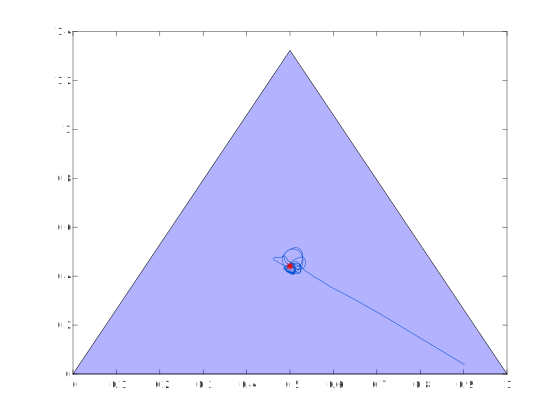
\includegraphics[width=7cm]{./img/rps_ewm.eps}
\caption{Rock Paper Scissor Dynamics in the $\Delta_2$ simplex, generated by the Exponentially Weighted Majority algorithm against an adversarial opponent.}
\label{fig:RPS}
\end{figure}

In Figure \ref{fig:RPS} we present the path of the randomization probabilities of the Rock Paper Scissor game represented in the $\Delta_{2}$ simplex, obtained by the Exponentially Weighted Majority algorithm against an adversarial opponent which plays the best response at each turn, knowing the probabilities of the learner.
Note that the algorithm learns to play the optimal strategy which is the randomization probabilities of $(1/3,1/3,1/3)$ over the action space. 
In general the dynamic of policies learned with Hanna consistent strategies are very complex and not well understood \cite{bailey2018multiplicative}.

\section{Online Convex Optimization for Regret Minimization}\label{sec:OCO}

Let us compare this framework to an apparently unrelated problem, namely optimization, that will turn out to be the most suited framework to embed the Online Portfolio Optimization Problem. In online optimization an agent $\mathcal A$ is designed to optimize a sequence of functions $f_t(x)$ where usually $f_t:\mathcal D\to \mathbb R$ is a real valued function from the set $\mathcal D\subset\mathbb R^n$. As a remark on the notation, in Online Convex Optimization literature, the loss functions are written as $f(x,y_t)\equiv f_t(x)$, dropping the explicit dependence on the outcome $y_t$.
The decision space $\mathcal D$ is assumed to be convex, as the functions $f_t:\mathcal D\to \mathbb R$. This framework was first devised in \cite{zinkevich2003online}, and has been later wildly used in the machine learning community to engineer optimization procedures \cite{shalev2012online}. 

Convexity plays a central role in most of the analysis made in Online Learning, and Online Convex Optimization. Convexity of the domain $\mathcal D$ and of the loss functions $f(\cdot,y)$ bounds the problem geometry and let us derive simple and efficient learning procedures.

In this chapter the decision space $\mathcal D$ is a convex subset of $\mathbb R^N$. As in the case of uncountable experts discussed in Section \ref{sec:uncountable_exp}, the best expert is the one who plays at each round a fixed point $x\in\mathcal D$. In Section \ref{sec:stat_learning} we will discuss how this framework is well suited to optimize complex functions, as Neural Networks, where we can think as $x\in\mathcal D$ as the set of parameters we are trying to optimize. Indeed many state of the art optimization techniques in the field of machine learning have been taking inspiration from the field of Online Optimization \cite{duchi2011adaptive}.

\subsection{A General Algorithm for Online Convex Optimization}\label{sec:OMD}

In this Section we will see an algorithm called \emph{Online Mirror Descent} (OMD), that generalizes many Online Convex Optimization algorithms. It is a first order method (\emph{i.e.} it uses only information from the gradient of the loss function) that works in the dual space defined by the choice of some regularizator. The OMD algorithm is general and optimal in the sense that every Online Convex problem can be learned online nearly optimally with OMD, the precise definition of the optimality of the OMD algorithm is quite complex to be summarized here and can be found in \cite{srebro2011universality}.

OMD works with a class of regularitators called Bregman Divergences, \cite{banerjee2005clustering}.

In this section we assume that $\mathcal D\subset \mathbb R^N$.

\begin{definition}(Bregman divergence). Given a differentiable convex function $\psi:\mathcal D\to\mathbb R$ the Bregman divergence is defined as an operator $d_{\psi}:\mathcal D\times\mathcal D\to \mathbb R^+$ defined for $\mathbf x,\mathbf y\in\mathcal D\times\mathcal D$ as: 
\begin{equation}\label{eq:bregman_div}
d_\psi(\mathbf x,\mathbf y)=\psi(\mathbf x)-\psi(\mathbf y)-\langle \mathbf x-\mathbf y,\nabla \psi(\mathbf y)\rangle.
\end{equation}
\end{definition}

Since $\psi$ is convex we have that $d_\psi(x,y)\ge0$. We can see that by linearization of $\psi(x)$ around $y\in\mathcal D$ and thanks to convexity the other terms are positive. However note that, since the operator defined in Equation \eqref{eq:bregman_div} is not symmetric in its arguments, it does not formally define a metric in the space $\mathcal D$.

Now we will present two example of Bregman divergences that we will use to define specifications of the OMD algorithm in Chapter \ref{ch:algos}.
For $\mathbf x,\mathbf y\in\Delta_{N-1}\subset \mathbb R^N$, consider $\psi(\mathbf x)=||\mathbf x||_2^2$ then the Bregman divergence becomes $d_\psi(\mathbf x,\mathbf y)=||\mathbf x-\mathbf y||_2^2$, which is the Euclidean norm. For $\psi(\mathbf x)=\sum\limits_{i=1}^Nx_i\log(x_i)$ then $d_\psi(\mathbf x,\mathbf y)=\sum\limits_{i=1}^Nx_i\log(x_i/y_i)$, which is the well know Kullback–Leibler divergence~\cite{van2014renyi}.

The OMD algorithm for Online Convex Optimization uses the regularization given by a Bregman divergence to follow the best point in the convex set $\mathcal D$ up to now, but it is kept close to the current one by the divergence operator. Formally:

\begin{definition}(Online Mirror Descent). OMD for a Bregamn Divergence induced by the differentiable, convex real values function $\psi$, and for a set of learning rates $\{\eta_0,\ldots,\eta_T\}$ has the following update rule: 

\begin{equation}\label{eq:OMD_update}
\mathbf x_{t+1} =\arginf\limits_{x\in\mathcal D} \left\{d_\psi(\mathbf x,\mathbf x_t)+\eta_t\langle\nabla f_t(\mathbf x_t),\mathbf x-\mathbf x_t\rangle\right\}.
\end{equation}
\end{definition}

Next we will show the idea for a general bound for the OMD algorithm, which explains the geometric ideas behind the OMD algorithm. Note that, in general, the analysis can be refined by fixing the loss function $f_t$ or the convex function $\psi$. \todo{F: questa frase invece non mi piace....direi invece

It is possible to show (citazione di dove c'è il teorema)
TEOREMA}

The convex function $\psi$ is assumed to be differentiable in the domain $\mathcal D$.

\begin{lemma}\label{th:OMD_first_th}
Let $d_\psi:\mathcal D\times\mathcal D\to \mathbb R$ the Bregman divergence associated to the convex smooth function $\psi$. Moreover, assume $\psi$ is $\alpha$-strong convex w.r.t. $||\cdot||$.
Then $\forall \mathbf x\in\mathcal D$ we have 
$$\eta_t (f_t(\mathbf x_t)-f_t(\mathbf x))\le d_\psi(\mathbf x,\mathbf x_t)-d_\psi(\mathbf x,\mathbf x_{t+1})+\frac{\eta_t^2}{2}||\nabla f_t(\mathbf x_t)||_*^2,$$ 
\end{lemma}

where we defined the dual norm $||\cdot||_*$ with respect to the norm $||\cdot||$.

\begin{definition}(Dual Norm).
Let $\mathbf x\in X$, the dual norm $||\cdot||_*$ of a norm $||\cdot||$ is defined as:
$$||\mathbf x||_*=\sup\limits_{\mathbf y:||\mathbf y||\le1}\langle \mathbf x,\mathbf y\rangle.$$
\end{definition}

The specific norm $||\cdot||$ in  Theorem \ref{th:OMD_first_th} can be chosen depending on the specific Bregman divergence, in order to simplify the analysis. Indeed, Theorem \ref{th:OMD_first_th} can be used to prove a regret bound for the general OMD algorithm. 

\begin{theorem}(Regret Bound for Online Mirror Descent).\label{th:regret_omd} Together with the assumptions of Theorem \ref{th:OMD_first_th} and if $\eta_t\ge0$ is a decreasing sequence of learning rates, then we have: 
$$R_T\le\max\limits_{t\le T}\frac{d_\psi(\mathbf x,\mathbf x_t)}{\eta_T}+\frac{1}{2\alpha}\sum\limits_{t=1}^T\eta_t||\nabla f_t(\mathbf x_t)||_*^2.$$
\end{theorem}


By choosing $\eta_t=\frac{D\sqrt{\alpha}}{\sqrt{\sum\limits_{t=1}^T||\nabla f_t(\mathbf x_t)||_*^2}}$, where $D=\max\limits_{t\le T}d_\psi(\mathbf x,\mathbf x_t)$, we have a bound for the OMD algorithm of 
\begin{equation}
R_T\le\frac{2D}{\sqrt\alpha}\sqrt{\sum\limits_{t=1}^T||\nabla f_t(\mathbf x_t)||_*^2}.
\end{equation}

Notice that, if the gradient under the dual norm is bounded by $||\nabla f_t(\mathbf x_t)||_*\le G\ \forall t\le T$, then we have that 
\begin{equation}
R_T\le\frac{2DG}{\sqrt\alpha}\sqrt T,
\end{equation}
which is sub-linear in $T$.

If $\eta_t=\eta>0$ is a constant sequence then Theorem \ref{th:regret_omd} can be simplified to give: 
\begin{equation}
R_T\le \frac{d_\psi(\mathbf x,\mathbf x_1)}{\eta}+\frac{\eta}{2\alpha}\sum\limits_{t=1}^T||\nabla f_t(\mathbf x_t)||^2_*.
\end{equation}

The OMD algorithm is a general technique to exploit the geometric convexity of the problem and gives rise to Hannan-consistent strategies in the case of uncountable convex decision spaces. By specializing the loss function and the Bregman divergences we can generate many algorithms that are state of the art in the Online Convex optimization problem, and achieve better theoretical guarantees than the general analysis we saw for the OMD algorithm, in fact we will show in Chapter \ref{ch:algos} that the Online Newton Step algorithm, which can be seen as an instance of the OMD algorithm, can achieve $\mathcal O(\log T)$ regret rather then $\mathcal O(\sqrt T)$ regret.

\begin{algorithm}[t!]
    \caption{OMD for Online Convex Optimization} 
    \label{alg:OMD_in_OCO}
    \begin{algorithmic}[1]
    \REQUIRE learning rate sequence $\{\eta_1, \ldots, \eta_T\}$  \nonumber
    \STATE Set $\mathbf{\mathbf x}_1 \gets \frac{1}{M} \mathbf{1}$ \label{line:init}
    \FOR {$t \in \{ 1, \ldots, T \}$}
    \STATE Observe $f_t(\mathbf x_t)$ decided by the adversary \label{line:out}
    \STATE $\mathbf x_{t+1} =\arginf\limits_{\mathbf x\in\mathcal D}\left\{ d_\psi(\mathbf x,\mathbf x_t)+\eta_t\langle\nabla f_t(\mathbf x_t),\mathbf x-\mathbf x_t\rangle\right\}$\label{line:update}
    \ENDFOR
    \end{algorithmic}
\end{algorithm}
\todo{F: manca riferimento nel testo e spiega}

\subsection{Mirror Version of the Online Mirror Descent Algorithm} 

The reason why OMD works is not that we are following the gradient, that points to the minimum of the function; indeed, the sub-gradient (Definition \ref{def:subgradient}) of a loss function does not point to the minimum in general (Figure \ref{fig_no_grad}). In practice the reason why OMD and other first order methods are effective is because of the convexity of the loss function and because of the following inequality for the instantaneous regret of convex loss functions:

\begin{figure}[!ht]
\begin{center}
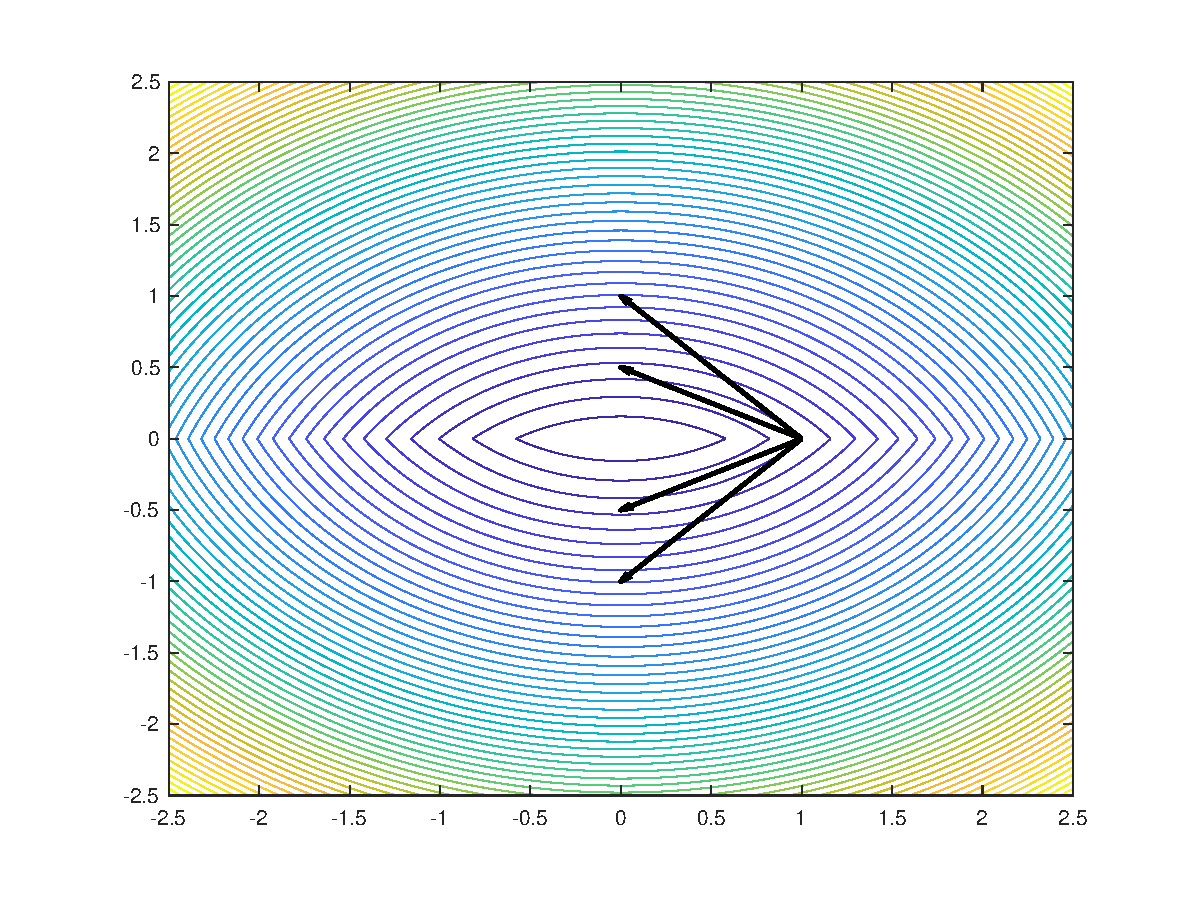
\includegraphics[width=4in,keepaspectratio]{./img/no_grad.eps}
\caption{Contour lines of $f(x,y)=\max\{x^2+(y-1)^2,x^2+(y+1)^2\}$, together with sub-gradient directions from $(1,0)$. All sub-gradient will point to increasing values of the function}
\label{fig_no_grad}
\end{center}
\end{figure}

\begin{equation}\label{eq:ineq_convex}
f_t(\mathbf x_t)-f_t(\mathbf x)\le\langle\nabla f_t(\mathbf x_t),\mathbf x_t-\mathbf x\rangle,
\end{equation}

and so to minimize the left hand side of Equation \eqref{eq:ineq_convex} we can minimize the right hand side of Equation \eqref{eq:ineq_convex}. Minimizing strictly a linear approximation of the instantaneous regret is not ideal since the environment is adversarial. Instead we minimize the linear approximation together with a regularization term which is given by the Bregman divergence $d_\psi$.

In order to understand more formally the inner workings of the OMD algorithm we have to introduce some concept from optimization theory:

\begin{definition}(Fenchel Conjugate).\label{def:fenchel_conj}
For a function $f:\mathbb R^N\to\mathbb R$ we can define the Fenchel conjugate as:

\begin{equation}
f^*(\mathbf \theta)=\sup\limits_{\mathbf x\in\mathbb R^N}\langle\mathbf x,\mathbf \theta\rangle -f(\mathbf x).
\end{equation}
\end{definition}

Definition \ref{def:fenchel_conj} can be interpreted as a generalized $\inf$ function as $f^*(\mathbf 0)$ is the classical $inf$ function. For $\mathbf x\neq\mathbf 0$ then we are looking for the infimum of the function $f$ when the axis of the function are rotated w.r.t. the hyperplane $H(\mathbf x)=\langle\mathbf\theta,\mathbf x\rangle$, as illustrated in Figure \ref{fig:fenchel}.

\begin{figure}[!ht]
\centering
\begin{pspicture}(0,-2.4522727)(6.540002,2.4522727)
\psline[linecolor=black, linewidth=0.04, arrowsize=0.05291667cm 2.0,arrowlength=1.4,arrowinset=0.0]{->}(1.7330438,-2.4522727)(1.7330438,2.3477273)
\psline[linecolor=black, linewidth=0.04, arrowsize=0.05291667cm 2.0,arrowlength=1.4,arrowinset=0.0]{->}(0.43304384,-1.5522727)(6.633044,-1.5522727)
\psbezier[linecolor=black, linewidth=0.016](0.033043824,2.0477273)(-0.06695618,-1.5522727)(3.3330438,-1.4522728)(3.3330438,2.0477272727272724)
\psline[linecolor=black, linewidth=0.016](0.43304384,-1.5522727)(4.986615,0.48234266)(5.533044,0.7477273)
\rput[bl](3.5875893,2.1022727){$f(\mathbf x)$}
\rput[bl](5.2603164,0.82045454){$\langle\mathbf x,\mathbf \theta\rangle$}
\psline[linecolor=black, linewidth=0.026](2.317031,-0.42408314)(2.4330437,-0.6522727)
\rput[bl](1.155266,-1.4856061){$\theta$}
\rput[bl](2.233044,-1.0078282){\textcolor{black}{$-f^*(\theta)$}}
\end{pspicture}
\caption{Fenchel Conjugate Function.}
\label{fig:fenchel}
\end{figure}


\begin{definition}(Sub-Gradient).\label{def:subgradient}
For a function $f:\mathbb R^N\to\mathbb R$ we can define the set of sub-differentials at $x_0$ as:
\begin{equation}
\partial f(x_0) = \{g : f(x)-f(x_0) \ge \langle g, x - x_0\rangle,\forall x\}.
\end{equation}
\end{definition}

For a differentiable at $\mathbf x_0$ function we have $\partial f(\mathbf x_0)=\{\nabla f(\mathbf x_0)\}$.

% The two concept clash together in the following theorem:

% \begin{theorem}(\cite{rockafellar1970convex}\label{th:fenchel_subdiff} Theorem 23.5). Let $f:\mathbb R^N\to\mathbb R$ be convex, then:
% \begin{equation}
% \mathbf x\in\partial f^*(\mathbb\theta) \iff \mathbb\theta\in \partial f^*(\mathbf x).
% \end{equation}
% \end{theorem}

% Theorem \ref{th:fenchel_subdiff} is fundamental to prove the following Theorem for OMD:

Finally, the following theorem explains the name of the OMD algorithm and its real more interesting formulation:

\begin{theorem}\label{th:OMD_mirror}
Let $d_\psi$ be a Bregman divergence operator then we have the following equality:

\begin{equation}
\arginf\limits_{\mathbf x\in\mathcal D}\{d_\psi(\mathbf x,\mathbf x_t)+\eta_t\langle\nabla f_t(x_t),\mathbf x-\mathbf x_t\rangle\}=\nabla \psi_{\mathcal D}^*(\nabla \psi(\mathbf x_t)-\eta_t\nabla f_t(\mathbf x_t)),
\end{equation}
where $\psi_\mathcal D$ is the restriction of $\psi$ to the convex set $\mathcal D$, \emph{i.e.,} $\psi_\mathcal D(\mathbf x)=\psi(\mathbf x)+\mathbb I^\infty_\mathcal D(\mathbf x)$, where we defined
\begin{equation*}
\mathbb I_\mathcal D^\infty(\mathbf x)=\begin{cases}
0&\text{if $\mathbf x\in\mathcal D$}\\
+\infty&\text{otherwise}.
\end{cases}
\end{equation*}.
\end{theorem}

% \begin{proof}(Sketch).
% The update rule of Equation \eqref{eq:OMD_update}:
% \begin{align}
% \mathbf x_{t+1}&=\arg\min\limits_{\mathbf x\in\mathcal D}\{d_\psi(\mathbf x,\mathbf x_t)+\eta_t\langle\nabla f_t(x_t),\mathbf x-\mathbf x_t\rangle\}\\
% &=\arg\min\limits_{\mathbf x\in\mathcal D}\langle\eta_t\nabla f_t(\mathbf x_t)-\nabla \psi(\mathbf x_t),\mathbf x\rangle+\psi(\mathbf x),
% \end{align}
% given 
% \end{proof}


Theorem \ref{th:OMD_mirror} shows the real nature of the OMD algorithm, which is to up{}date predictions using the gradient of the loss function, in the dual space defined by the function $\psi$. For example if $\psi(\mathbf x)=\frac{1}{2}||\mathbf x||_2^2$ then we have $\nabla \psi(\mathbf x_t)=\mathbf x_t$ and $\nabla \psi^*(\mathbf x)=\Pi_\mathcal D(\mathbf x)$, and we obtain the Online Gradient Descent algorithm, $\mathbf x_{t+1}=\Pi_\mathcal D(\mathbf x_t-\eta_t\nabla f_t(\mathbf x_t))$, that we will explore with detail in Chapter \ref{ch:OGD}.

\begin{figure}[!ht]
\centering
\begin{pspicture}(0,-2.316111)(8.93147,2.316111)
\psbezier[linecolor=black, linewidth=0.026](4.2682414,-0.4629235)(4.253908,0.08388889)(6.244009,2.449626)(7.3191204,2.017222222222222)(8.394232,1.5848185)(9.182215,0.0771305)(8.653908,-0.7344378)(8.125602,-1.5460061)(5.6539083,-1.4161111)(5.178153,-1.2716666)(4.7023973,-1.1272222)(4.282575,-1.009736)(4.2682414,-0.4629235)
\pstriangle[linecolor=black, linewidth=0.026, dimen=outer](1.5094637,-1.2716666)(3.0,2.6111112)
\psbezier[linecolor=black, linewidth=0.026, arrowsize=0.05291667cm 2.0,arrowlength=1.4,arrowinset=0.0]{->}(1.4539081,0.3838889)(1.8292384,2.1910827)(6.1724277,2.3313398)(6.453908,0.9838888888888868)
\rput[bl](1.2316859,1.2838889){$\mathcal D$}
\rput[bl](3.8094637,2.0061111){$\nabla \psi$}
\psbezier[linecolor=black, linewidth=0.026, arrowsize=0.05291667cm 2.0,arrowlength=1.4,arrowinset=0.0]{->}(5.353908,-0.8161111)(4.6871533,-1.9411111)(1.253908,-2.2161112)(1.253908,-1.0161111111111132)
\rput[bl](3.1205747,-2.316111){$\nabla \psi^*$}
\rput[bl](1.2872415,0.07277778){$\mathbf x_t$}
\rput[bl](1.2316859,-0.88277775){$\mathbf x_{t+1}$}
\rput[bl](6.7101727,0.7838889){$\nabla\psi(\mathbf x_t)$}
\psline[linecolor=black, linewidth=0.026, arrowsize=0.05291667cm 2.0,arrowlength=1.4,arrowinset=0.0]{->}(6.453908,0.8838889)(5.6761303,-0.49388888)
\rput[bl](6.220575,-0.016111111){$\eta_t\nabla f_t(\mathbf x_t)$}
\rput[bl](4.9333954,-0.77508545){$\nabla\psi(\mathbf x_t)-\eta\nabla f_t(\mathbf x_t)$}
\end{pspicture}
\caption{Online Mirror Descent as Mirror Updates.}
\label{fig:OMD_mirror}
\end{figure}



\section{From Online Learning to Statistical Learning}\label{sec:stat_learning}
Now we explore the connection between the Online Optimization framework and classical concepts of classical Statistical Learning techniques. More concretely we can prove and design a whole class of algorithms that are Agnostically PAC Learnable with Online Learning Techniques. \todo{define PAC}
Classical statistical learning theory deals with examples (or observations) and models of the phenomena. Then it uses the model to predict the future observations~\cite{bousquet2003introduction}. Quite informally one could say that we are trying to infer concept from examples. A concept is a map $\mathcal C:\mathcal D\to\mathcal Y$, where $\mathcal D$ is the domain space and $\mathcal Y$ is the set of labels for the examples. We then observe a sample from an unknown distribution $\mathcal X$ such that $(x,y)\sim \mathcal X$. What we need to achieve is to learn a mapping $y:\mathcal D\to\mathcal Y$ such that the error under the distribution $\mathcal X$ is small. The loss function needed to define this error is not specific to the problem and can be decided by the user. This is called generalization error and, for a loss function $l:\mathcal Y\times\mathcal Y \to\mathbb R$, it is defined as:
\begin{equation}\label{eq:generalization}
    e(h) = \mathbb E_{(x,y)\sim \mathcal X}[l(h(x),y)].
\end{equation}
The goal for an algorithm $\mathcal A$ is to produce a hypothesis $h$ with small generalization error. 
In general, it is difficult to obtain small generalization error and how difficult it is clarified by the following theorem called the \emph{No free lunch theorem} \cite{mitchell1997machine}.
This restriction gives raise to the concept of Probably Approximately Correct (PAC) learnability. 

\begin{definition}(PAC learnable).\label{def:PAC}
    An hypothesis class $\mathcal H$ is PAC learnable w.r.t. the loss $l$ if there exists a learner $\mathcal A$ that given a sample $S_N$ of examples learns an hypothesis $h\in\mathcal H$ s.t. for all $\epsilon,\delta$ there exists $N_{\epsilon,\delta}$ such that for any distribution $\mathcal D$ we have a generalization error s.t. $\mathbb P\left[e(h)<\epsilon\right]\ge1-\delta$.
\end{definition}

Usually, we also require that the algorithm $\mathcal A$ learns the concept $h$ in polynomial time w.r.t. the parameter of the problem. 

An example of such learning problems could be the classification of spam emails. In this case $\mathcal D$ is the vectorial representation of the text and $\mathcal Y=\{0,1\}$, indicating weather or not the email is a spam or not. If we choose as a model a linear classifier then the hypothesis space is $\mathcal H=\{h = \mathbb I[\langle x,w\rangle \ge 1/2]\}$ and the loss could be chosen as $l(y_1,y_2)=|y_1-y_2|$.

PAC learnability intuitively requires the existence of an hypothesis $h\in\mathcal H$ with near zero generalization error, otherwise the class $\mathcal H$ is not PAC learnable.
But we can weaken the concept of PAC learnability by addressing directly this issue.

\begin{definition}(PAC agnostic learnable).
    Given the same definitions of Definition \ref{def:PAC}, an hypothesis class $\mathcal H$ is PAC agnostic learnable if we have a generalization error s.t. $\mathbb P\left[e(h)<\inf\limits_{\tilde h\in\mathcal H}e(\tilde h)+\epsilon\right]\ge1-\delta.$
\end{definition}

Determining which hypothesis spaces $\mathcal H$ are PAC learnable (agnostically or not) for specific spaces is an open and complex issue, but the case for convex hypothesis class $\mathcal H\subset\mathcal R$ can be solved by Online Learning techniques, showing the versatility of the methods. 
Moreover, the approach to prove such theorem gives a constructive methodology to solve agnostic PAC learnable problems.

\begin{theorem}\todo{cit theorem}
For every hypothesis class $\mathcal H$ and bounded loss function $l:\mathcal Y\times\mathcal Y\to \mathbb R$, for which does exists a low regret algorithm $\mathcal A$, the problem is agnostic PAC learnable. In particular, these conditions are satisfied if the hypothesis space $\mathcal H$ and the loss function $l$ are convex.
\end{theorem}

\begin{proof}(Sketch).
Initialize the learner with the hypothesis $h_0=\mathcal H$.
For every iteration $t\le T$: observe a sample $(x_t,y_t)\sim\mathcal X$ and a loss function $l_t:=l(h_t(x_t),y_t)$. Then update the hypothesis $h_{t+1}=\mathcal A(l_1,\ldots,l_t)$.

At $t=T$ return $\bar{h}=\frac{1}{T}\sum\limits_{t=1}^T h_t\in\mathcal H$. 

The proof then continues by defining the random variable $X^{(1)}_T=\sum\limits_{t=1}^Te(h_t)-l(h_t(x_t),y_t)$. This is a martingale and $\mathbb E[X^{(1)}_T]=0$. Moreover $|X^{(1)}_T-X^{(1)}_{T-1}|<K$ since the loss function $f$ is bounded. We can normalize the losses so that $K=1$, and then apply the Azuma martingale inequality $\mathbb P[X^{(1)}_T>c]\le e^{-\frac{c^2}{2T}}$ \cite{azuma1967weighted}.

For an appropriate choice of $c$ we get

\begin{equation}\label{eq:ineq_1_APCA}
\mathbb P\left[\frac{1}{T}\left[\sum\limits_{t=1}^Te(h_t)-l(h_t(x_t),y_t)\right)>\sqrt{\frac{2\log(\delta/2)}{T}}\right]\le \delta/2,
\end{equation}
defining $h^*=\arginf\limits_{h\in\mathcal H} e(h)$ and $X^{(2)}_T=\sum\limits_{t=1}^Te(h^*)-l(h^*(x_t),y_t)$ we can obtain
\begin{equation}\label{eq:ineq_2_APCA}
\mathbb P\left[\frac{1}{T}\left(\sum\limits_{t=1}^Te(h^*)-l(h^*(x_t),y_t)\right)<-\sqrt{\frac{2\log(\delta/2)}{T}}\right]\le \delta/2.
\end{equation}

By the definition of regret $R_T$ we obtain

\begin{equation}\label{eq:eq_regret_APAC}
\frac{1}{T}\sum\limits_{t=1}^Te(h_t)-e(h^*)=R_T/T+X_T^{(1)}-X_T^{(2)},
\end{equation}

and from inequalities in Equations \eqref{eq:ineq_1_APCA}, \eqref{eq:ineq_2_APCA} and from Equation \eqref{eq:eq_regret_APAC} we have:

\begin{equation}
\mathbb P\left[\frac{1}{T}\sum\limits_{t=1}^Te(h_t)-e(h^*)>\frac{R_T}{T}+2\sqrt{\frac{2\log(\delta/2)}{T}}\right]\le \delta.
\end{equation}

Now simply thanks to the linearity of the error operator $e:\mathcal H\to \mathbb R$ we have that 

\begin{equation*}
\mathbb P\left[e(\bar h)<e(h^*)+R_T/T+2\sqrt{\frac{2\log(\delta/2)}{T}}\right]\le 1-\delta,
\end{equation*}
and since $R_T/T\to0$ we can find $\tilde T$ large enough such that the thesis is verified.
\end{proof}

This result has been presented since it is useful to prove the general behavior of Hannan-consistent strategies in environments driven by a stationary distribution.
\chapter{Information, Prediction and Investing}

In Chapter \ref{ch:OnlineLearning} we described at a high level the framework of Online Learning in Adversarial environment. Now we draw the connections between that and predictions. It surly seems counter intuitive to speak about predictions in an adversarial framework, since we are used to think about predictions only of stochastic processes. The root of this formulation are to be traced back to the Bell Laboratories in the '50, from works of Kelly \cite{kelly2011new}, linking sequential betting and information rate. This connection is of primary importance to understand sequential investing as an instance of sequential decision problem.
We first draw the parallelism between probability assignment over discrete events and Online Learning and then extend the discussion to sequential investments.

\section{Probability assignment}
The decision space $\mathcal D$ in the case of finite $N$ possible bets is the $\Delta_{N-1}\subset \mathbb R^{N}$ probability simplex while the outcome $\mathcal Y$ space is the set $\{1,\ldots,N\}$, representing the winning bet at each turn. The loss function $f(x,y)$ should have these natural properties: low when $x_y~1$ and high when $x_y~0$ where $x_y$ is the probability assigned to the outcome $y$. The inverse log-likelihood seems a reasonable proposal, simply because the multiplicative additive property of the logarithm but has also a deeper connection to information that we will discuss later on:

\begin{definition}(Self Information Loss).
    In the sequential probability assignment problem the loss function $f(x,y)$, $x\in \Delta_{N-1}$ and $y\in[1,\ldots,N]$ is defined as
    $$f(x,y)=-\log(x_y)$$
where $x_y$ is the probability assigned to outcome $y\in\mathcal Y$.
\end{definition}

In the case of simulable experts, the prediction $x_t$ of the agent is a function of the history of outcomes $y^{t-1}:=\{y_1,y_2,\ldots,y_{t-1}\}\in\mathcal Y^{t-1}$. An expert can be thought of as a set of functions $g_k:\mathcal Y^{k-1}\to\Delta_{N-1}$.




\chapter{Algorithms for the Online Portfolio Optimization Problem}

In this section we will review the state of the art algorithms for the Online Portfolio Optimization problem and discuss their theoretical guarantees.


\chapter{Algorithms for the Online Portfolio Optimization Problem}\label{ch:algos}

In this section we will review the state of the art algorithms for the Online Portfolio Optimization problem and discuss their theoretical guarantees, and how this algorithms can be generated by the theoretical framework of Online Learning with expert advice and Online Optimization we described in Chapter \ref{ch:OnlineLearning}.

The setting is the one described in Section \ref{sec:OPO}, in particular $\Delta=\Delta_{N-1}\subset \mathbb R^N$ is the $N$-simplex, and an element $\mathbf x_t\in\Delta$ describes the allocation into $N$ stocks for the $t$-th period.

As is commonly done in the portfolio allocation literature~\cite{agarwal2006algorithms}, we assume that the price of the assets does not change too much during two consecutive rounds, or, formally:

\begin{assumption} \label{ass:nojunk}
    %  Given the OPO framework, 
     There exist two finite constants $\epsilon_l, \epsilon_u \in \mathbb{R}^+$ s.t.~the price relatives~$y_{j,t} \in [\epsilon_l, \epsilon_u]$, with $0 < \epsilon_l \leq \epsilon_u < +\infty$, for each round $t \in \{ 1, \ldots, T \}$ and each asset $j \in \{1, \ldots, N \}$.
\end{assumption}

Notice that under Assumption~\ref{ass:nojunk}, it is possible to bound the $L_1$, $L_2$ and the $L_\infty$ gradient of the loss as follows:\todo{check}

\begin{equation} \label{eq:bounded_gradient}
    ||\nabla \log (\langle \mathbf{x}_t, \mathbf{y}_t) \rangle||_1 \leq \frac{N\epsilon_u}{\epsilon_l}:=G_1.
\end{equation}

\begin{equation} \label{eq:bounded_gradient}
    ||\nabla \log (\langle \mathbf{x}_t, \mathbf{y}_t) \rangle||_2 \leq \frac{\epsilon_u \sqrt{N}}{\epsilon_l}:=G_2.
\end{equation}

\begin{equation} \label{eq:bounded_gradient}
    ||\nabla \log (\langle \mathbf{x}_t, \mathbf{y}_t) \rangle||_\infty \leq \frac{\epsilon_u }{\epsilon_l}:=G_\infty.
\end{equation}

Since we will compare multiple algorithms we introduce the notation: $R_T(\mathcal A)$, when speaking about the regret at time $T$ of an online learner $\mathcal A$, the same notation applies with the total regret $R_T^C$ or the regret on the costs $C_T$, defined in Section \ref{ch:transaction_costs}.

\section{Algorithm with regret bound}

As already pointed out, most algorithms in the Online Portfolio Optimization literature do not consider transaction costs and have guarantees only on the standard regret $R_T$. In this section we will summarize the most relevant algorithms for the Online Portfolio Optimization problem that have been proven to have only bounded regret $R_T$. 

\subsection{Universal Portfolios}\label{sec:UP}
The Universal Portfolios (UP) \cite{cover1996universal} algorithm has the best theoretical guarantees among the algorithm for Online Portfolio Optimization. 

\begin{definition}(Universal Portfolios).
\begin{equation}\label{eq:UP}
\mathbf x_{t+1}=\frac{\int_{\Delta}\mathbf x W_t(\mathbf x)d\mathbf x}{\int_{\Delta} W_t(\mathbf x)d\mathbf x}.
\end{equation}
\end{definition}

Note that this algorithm is the Continuous Mixture Forecaster for exp-concave losses, described in Section \ref{sec:exp-concave-mixture}, since the logarithmic loss is exp concave with $\nu=1$. With the analysis described in Section \ref{sec:laplace_mixture}.

Hence we have that 
\begin{equation}
R_T(UP)\le(N-1)\log(T+1).
\end{equation}

Clearly, the UP algorithm is computationally hard as it involves integration over a $N$-simplex. Indeed, there is an extensive research that looks into efficient implementations of the UP algorithm \cite{kalai2002efficient}.

Equation \eqref{eq:UP} can be refined with:

\begin{equation}\label{eq:general_UP}
\mathbf x_{t+1}=\frac{\int_{\Delta}\mathbf x W_t(\mathbf x)\mu(\mathbf x)d\mathbf x}{\int_{\Delta} W_t(\mathbf x)\mu(\mathbf x)d\mathbf x},
\end{equation}

where $\mu(\mathbf x)$ is a distribution over $\Delta_{N-1}$, there are choices of $\mu(\mathbf x)$ for which we can obtain slightly better constants for the regret bound.


\subsection{Exponential Gradient}

The Exponential Gradient (EG) algorithm is a specification of the OMD algorithm described in Section \ref{sec:OMD}, by using as the Bregman divergence the Kullback–Leibler divergence $d_\psi(\mathbf x,\mathbf y)=KL(\mathbf x,\mathbf y)=\sum\limits_{i=1}^Nx_i\log(x_i/y_i)$, and $\eta_t=\eta$ as constant sequence of learning rates. The update rule for EG in this case becomes:

\begin{definition}(Exponential Gradient).
\begin{equation}\label{eq:update_EG}
\mathbf x_{t+1}=\arg\min\limits_{x\in\Delta_{N-1}} KL(\mathbf x,\mathbf x_t)-\eta_t\left\langle \frac{\mathbf x_t}{\langle \mathbf x_t,\mathbf y_t\rangle},\mathbf x-\mathbf x_t\right\rangle.
\end{equation}
\end{definition}

The update rule in Equation \eqref{eq:update_EG} can be solved analytically \cite{helmbold1998line}, giving the following closed update 

\begin{equation}\label{eq:update_EG_closed}
x_{i,t+1}=\frac{x_{j,t}\exp\left(\eta_t{y_{j,t}}/\langle\mathbf x_t,\mathbf y_t\rangle\right)}{\sum\limits_{j=1}^Nx_{j,t}\exp\left(\eta_t{y_{j,t}}/\langle\mathbf x_t,\mathbf y_t\rangle\right)}, \forall i\in1,\ldots,N.
\end{equation}

This update rule is also of the kind of an Weighted Average Forecaster described in Section \ref{sec:existence_of_no_regret}, in particular it is a special kind of Exponentially Weighted Forecaster of Definition \ref{def:ewf}.

We know that $\psi(\mathbf x)=\sum\limits_{i=1}^Nx_i\log(x_i)$ is $1$-strong convex with respect to the $L_1$ norm $||\cdot||_1$ \cite{shalev2007online}, and so we have that $KL(\mathbf x,\mathbf x_t)\ge\frac{1}{2}||\mathbf x-\mathbf x_t||_1$.

Moreover, we we can bound the $L_1$ diameter $D_1$ of the simplex $\Delta_{N-1}$ as: 
$$D_1=\sup\limits_{\mathbf x,\mathbf y\in\Delta_{N-1}}||\mathbf x-\mathbf y||_1\le2.$$

Therefore, we can apply straightforward Theorem \ref{th:regret_omd} with $\eta=\frac{1}{G_\infty}\sqrt{\frac{2\log N}{T}}$ and $\mathbf x_1=(1/N,\ldots,1/N)$ giving as a result the following regret bound:

\begin{equation}
R_T(EG)\le \frac{\epsilon_u}{\epsilon_l}\sqrt{\frac{T\log N}{2}}.
\end{equation}


\subsection{Online Newton Step}

The Online Newton Step (ONS) \cite{hazan2007logarithmic} algorithm is one of the few algorithm other than the UP algorithm that guarantees a logarithmic bound $R_T(ONS)=\mathcal O(\log T)$. The method uses second order information of the loss function, but it can nonetheless stated into first order method such as OMD. 

\begin{definition}(Online Newton Step).
\begin{equation}\label{eq:update_ONS}
\mathbf x_{t+1}=\Pi^{A_t}_{\Delta_{N-1}}\left(\mathbf x_t+\frac{1}{\beta}A_t^{-1}\frac{\mathbf y_t}{\langle\mathbf x_t,\mathbf y_t\rangle}\right),
\end{equation}
where $\prod^{A_t}_{\Delta_{N-1}}$ is the non-standard projection onto the simplex $\Delta_{N-1}$ defined as 
$$\Pi^{A_t}_{\Delta_{N-1}}(\mathbf x_0):=\arg\inf\limits_{\mathbf x\in\Delta_{N-1}}\langle\mathbf x-\mathbf x_0,A_t(\mathbf x-\mathbf x_0)\rangle.$$

and the matrix $A_t\in\mathbb R^{N\times N}$ it is defined as $A_t=\sum\limits_{s=1}^t \nabla f_t(\mathbf x_t)\nabla f_t(\mathbf x_t)^T+\epsilon\mathbb I_N$.
\end{definition}

The idea for the ONS algorithm is originated from the concept of strong convexity, that is defined as follow:

\begin{definition}(Strong Convexity).\label{def:strong_cnvx}
A function $f:\mathcal D\to\mathbb R$ is said to be $\mu$-strong convex w.r.t. the norm $||\cdot||$ if: 
$$f(y)-f(x)\ge\langle\nabla f(x),y-x\rangle+\frac{\mu}{2}||y-x||^2,\forall x,y\in\mathcal D,\forall x,y\in\mathcal D.$$
\end{definition}

Usually there is the correspondence of convex-loss $R_T=\mathcal O(\sqrt T)$ and strong-convex loss $R_T=\mathcal O(\log T)$. The idea of the ONS algorithm is to recover a weaker concept of strong convexity for exp-concave losses:

\begin{definition}(Weak Strong Convexity).\label{def:weak_strong_cnvx}
A function $f:\mathcal D\to\mathbb R$ is said to be weak-strong convex if $\forall x\in\mathcal D\exists A$ such that: 
$$f(y)-f(x)\ge\langle\nabla f(x),y-x\rangle+\frac{\mu}{2}||y-x||_{A}^2,$$
for a matrix $A$ that defines the norm $||x||^2_{A}=\langle x, Ax\rangle$.
\end{definition}

In fact for any $\nu$ exp-concave function $f:\mathcal D\to\mathbb R$ with bounded gradient, \emph{i.e.} $||\nabla f(\mathbf x)||_2\le G\ \forall \mathbf x\in\mathcal D$, with $D=\sup\limits_{\mathbf x,\mathbf y\in\mathcal X}||\mathbf x-\mathbf y||_2$, $\beta=\frac{1}{2}\min\{\nu,\frac{1}{4GD}\}$ and $A=\nabla f(\mathbf x)\nabla f(\mathbf x)^T$, we have that: 

\begin{equation}\label{eq:weak_strong_conv_exp_concave}
f(\mathbf y)-f(\mathbf x)\ge\langle\nabla f(x),\mathbf y-\mathbf x\rangle+\frac{\beta}{2}||\mathbf y-\mathbf x||_{A}\forall x,y\in\mathcal D.
\end{equation}

The main idea of ONS exploit the weak-strong convexity of exp-concave functions to recover $\mathcal O(\log T)$ regret bounds, the complete proof can be found in \cite{hazan2007logarithmic}.

From Equation \eqref{eq:weak_strong_conv_exp_concave} we can see that the matrix $A_t$ used by the ONS algorithm is just a lower bound on the Hessian of the loss function. This is also why the projection onto the simplex of the ONS algorithm is the non standard projection defined by the matrix $A_t$.

Finally, choosing $\beta=\frac{\alpha}{8\sqrt{N}}$ the regret bound for the ONS algorithm becomes:

\begin{equation}\label{eq:regret_ONS}
R_T(ONS)\le\frac{10 N^{3/2}}{\epsilon_l}\log\left(\frac{NT}{\epsilon_l^2}\right)
\end{equation}

\section{Algorithm with total regret bound}

To the best of our knowledge there are only two works that bound the total regret bound $R_T^C$ defined in Chapter \ref{ch:transaction_costs}. We will present the works and discuss their limitations, that we tried to solve with our approach.

\subsection{Online Lazy Updates}

Online Lazy Updates (OLU) \cite{das2013online} is an algorithm designed to minimize explicitly the total regret $R_T^C$. The origin of this algorithm has to be traced back to a generalization of the OMD algorithm discussed in Section \ref{sec:OMD}. Namely, the generalization of the OMD algorithm that we are referring to, is the Composite Objective Mirror Descent (COMID) algorithm \cite{duchi2010composite}. The idea behind the COMID algorithm is the have a composite loss function of the kind $g_t(\mathbf x)=f_t(\mathbf x) + r(\mathbf x)$, then the algorithm linearizes the first term $f_t(\mathbf x)$ of the composite loss (as in OMD), but does not linearize the second term $r(\mathbf x)$ of the composite loss $g_t(\mathbf x)$. Both terms of the loss function, $f_t$ and $r$, are assumed to be convex.

\begin{definition}(Composite Objective Mirror Descent).\label{def:COMID}
\begin{equation}\label{eq:update_COMID}
    \mathbf{x}_{t+1}=\arg \hspace{-0.1cm} \min\limits_{\mathbf{x} \in \Delta_{M-1}} \hspace{-0.1cm} \left\{ \eta \langle \nabla f_t(\mathbf{x}_t), \mathbf{x} \rangle + \eta \ r(\mathbf{x}) + d_\psi(\mathbf{x}, \mathbf{x}_t) \right\},
\end{equation}

Where $d_\psi$ is the Bregman divergence for a convex function $\psi$. 

\end{definition}

A lemma similar to Lemma \ref{th:OMD_first_th} gives the following guarantees to the regret of a learner using COMID:

\begin{lemma}(\cite{duchi2010composite} Theorem 2.2)
$\forall \mathbf x\in\Delta_{N-1}$ and for a sequence $\{\mathbf x_t\}_{t=1}^T$ defined by the update rule \eqref{eq:update_COMID}, we have:
\begin{equation}
\eta\sum\limits_{t=1}^T[f_t(\mathbf x_t)-f_t(\mathbf x)+r(\mathbf x_t)-r(\mathbf x)]\le d_\psi(\mathbf x,\mathbf x_t)+\eta r(\mathbf x_1)+\frac{\eta^2}{2\alpha}\sum\limits_{t=1}^T||\nabla f_t(\mathbf x_t)||_*^2,
\end{equation} 
where $\alpha$ is the parameter that ensures $d_\psi(\mathbf x,\mathbf y)\ge \frac{\alpha}{2}||\mathbf x-\mathbf y||^2$.
\end{lemma}

This lemma implies easily regret bound on the regret $R_T$. If we assume that the losses $f_t$ have bounded gradient by $G_*$ under the norm $||\cdot||_*$ then we have that: 

\begin{equation}
\sum\limits_{t=1}^T[f_t(\mathbf x_t)-f_t(\mathbf x)+r(\mathbf x_t)-r(\mathbf x)]\le\frac{1}{\eta}d_\psi(\mathbf x,\mathbf x_t)+r(\mathbf x_1)+\frac{T\eta}{2\alpha}G_*^2.
\end{equation}

Consequently, taking $\eta=\frac{K}{\sqrt T}$ we obtain, and assuming $d_\psi(\mathbf x,\mathbf y)\le D\ \forall\mathbf x,\mathbf y\in\Delta_{N-1}$, and assuming $r(\mathbf x_1)\le D_1$ we obtain:

\begin{equation}\label{eq:regret_comid_final}
\sum\limits_{t=1}^T[f_t(\mathbf x_t)-f_t(\mathbf x)+r(\mathbf x_t)-r(\mathbf x)]\le KD\sqrt{T} + D_1+\frac{\sqrt{T}}{2\alpha}G_*^2.
\end{equation}

The idea of OLU is to take $r=r_t(\mathbf x)=\gamma||\mathbf x-\mathbf x_{t-1}||_1$ \cite{das2014online}, $\psi=||\mathbf x||_2^2$ generating the following update rule:

\begin{definition}(Online Lazy Update).\label{def:update_OLU}
\begin{equation}\label{eq:update_COMID}
    \mathbf{x}_{t+1}=\arg \hspace{-0.1cm} \min\limits_{\mathbf{x} \in \Delta_{M-1}} \hspace{-0.1cm} \left\{ -\eta\log(\langle \mathbf x,\mathbf y_t\rangle) + \eta \gamma ||\mathbf x_t-\mathbf x||_1 + \frac{1}{2}||\mathbf x-\mathbf x_t||^2_2 \right\},
\end{equation}

\end{definition}

Note that there are multiple definitions of the OLU algorithm, and we reported a version in which the first term of the loss has note been linearized. Linearization of the first term of the loss with $\langle\nabla f_t(\mathbf x_t),\mathbf x\rangle$ would results in the same update rule and same analysis (since the loss $f_t$ is convex).

With this specifications we obtain the result from \eqref{eq:regret_comid_final}:

\begin{equation}
\sum\limits_{t=1}^T[f_t(\mathbf x_t)-f_t(\mathbf x)+\gamma||\mathbf x_t-\mathbf x_{t-1}||_1-\gamma||\mathbf x-\mathbf x_{t-1}||_1]\le \left( \frac{1}{K} + \frac{N K \epsilon_u^2 }{2 \epsilon_l^2} \right) \sqrt{T}.
\end{equation}

Then taking to the left hand side the terms $\gamma||\mathbf x-\mathbf x_{t-1}||_1$, and specializing $f_t(\mathbf x)$ as the log-loss defined for the Online Portfolio Optimization framework, we obtain:

\begin{equation}
\sum\limits_{t=1}^T[f_t(\mathbf x_t)-f_t(\mathbf x)+\gamma||\mathbf x_t-\mathbf x_{t-1}||_1]\le \sum\limits_{t=1}^T\gamma||\mathbf x-\mathbf x_{t-1}||_1+\left( \frac{1}{K} + \frac{N K \epsilon_u^2 }{2 \epsilon_l^2} \right) \sqrt{T}.
\end{equation}

Now the left hand side is equivalent to our Definition \ref{def:totoal_regret} of total regret $R_T^C$. Note that we do not have a sub-linear bound for the total regret yet. In order to recover the sub-linear bound on the total regret $R_T^C$ in \cite{das2014online} (Theorem 1) the authors assume $\gamma=\frac{K'}{\sqrt{T}}$. With this assumption we can recover the following bound on the total regret for the OLU algorithm:

\begin{equation}
R_T^C(OLU)\le2K'\sqrt{T}+\left( \frac{1}{K} + \frac{N K \epsilon_u^2 }{2 \epsilon_l^2} \right) \sqrt{T}.
\end{equation}

It is clear from our discussion on the model for Online Portfolio Optimization with transaction costs described in Chapter \ref{ch:transaction_costs}, that $\gamma>0$ is fixed and independent on the time horizon $T$ of the investment process. \todo{magari mettere quelsta discussione su OLU come th?}


\subsection{Universal Portfolios with Transaction Costs}

In \cite{blum1999universal} the authors extended the ideas of the UP algorithm \ref{sec:UP} to include transaction costs. The approach is heavily inspired by the results in Online Learning of Section \ref{sec:laplace_mixture}, namely, the Laplace Mixture Forecaster for the log-loss, and it differs substantially with our approach that is inspired by the Online Convex Optimization framework.

Indeed the Laplace mixture forecaster has the property \cite{cover1996universal} that the wealth of the Laplace Mixture Forecaster is the average wealth of the wealth of the expert class. The idea followed by the authors is to show that is the portfolios in the expert class are paying transaction costs then the regret experienced by the algorithm \todo{vorrei non mettere UCP perché non lo capisco}

\section{Other Related Works}

There are also heuristic algorithms designed to exploit some known phenomena in markets. Among these heuristic algorithm we can find, Anticor~\cite{borodin2004can}, PAMR~\cite{li2012pamr}, OLMAR~\cite{li2015moving}, and MRTC~\cite{yang2018reversion}, which in some cases outperform the algorithms described above in terms of empirical performance. 
Remarkably, none of the above algorithms provide guarantees on the regret, and so we will avoid an in depth description of their mechanism, since we are currently concerned with algorithm that provide theoretical guarantees without assumptions on the distribution of the marker vectors.

\todo{rephrase}
\chapter{Online Gradient Descent for Online Portfolio Optimization with Transaction Costs}

The Online Gradient Descent (OGD) algorithm is the first algorithm developed in the field of Online Convex Optimization \cite{zinkevich2003online}. We extended its use to the Online Portfolio Optimization framework, this will be discussed more in details in . \todo{add ch} \todo{continue}
\chapter{Numerical Experiments} 
\label{ch:experiments}

In this section we analyze the empirical performance of OGD, comparing it with the algorithm from the Online Portfolio Optimization literature that provides guarantees on total regret: OLU~\cite{das2013online}.
We also consider UP~\cite{cover1996universal} and ONS~\cite{agarwal2006algorithms}, because UP\footnote{
We used a na\"ive version of UP since the classic implementation required an unfeasible amount of time for the experiments.
Instead, we discretized the simplex with $10^4$ points and used the corresponding CRPs to approximate the integrals used by UP.} has the best theoretical guarantees on the regret $R_T$ and ONS because has both good theoretical guarantees on the regret on the wealth $R_T$ and is known to provide the best results regarding the regret on the wealth when analyzed empirically.

\begin{table}[ht!]\centering
\begin{tabular}{ |c||c|c|c|c| }
 \hline
 \multicolumn{5}{|c|}{Datasets} \\
 \hline
 Name & Market &Year Span & Rebalances & Assets\\
 \hline
 NYSE(O) & New York Stock Exchange  & 1962 - 1984  &5651&   36\\
 TSE & Toronto Stock Exchange & 1994 - 1998  & 1258   &88\\
 SP500 & Standard Poor's 500 & 1998 - 2003 & 1276&  25\\
 \hline
\end{tabular}
\caption{Description of the main datasets used that common in the Online Portfolio Optimization literature.}\label{tab:dataset}
\end{table}

Table \ref{tab:dataset} summarizes the datasets used for the experiments. All assets in the datasets are being anonymize to ensure to avoid common bias toward specific assets.
To compare the algorithms, we used mainly the NYSE(O) dataset, a well-known benchmark that has been previously used in several portfolio optimization research papers, and notably, in all the works which propose the algorithms here considered as baselines.
The NYSE(O) dataset spans $22$ years (between $1962$ and $1984$), for a total investment horizon of $T = 5651$ days ($\approx250$ working days per year).
In each experiment, we sampled a set of $N=5$ assets randomly chosen among the $36$ and ran the algorithms for the entire investment horizon $T$.
We ran $100$ independent experiments for the NYSE(O) datasets, $20$ and $50$ for the TSE and SP500 dataset respectively, and then we averaged the results. The choice of doing a great number of experiments is to stress the point that we are not concerned with the selection of assets to invest in, but only with the behavior of the algorithms with respect to transaction costs.
We considered different values for the transaction rate $\gamma \in \{ 0, 0.0005, 0.001, 0.003, 0.006, 0.01, 0.02, 0.04 \}$, including hight values of $\gamma$ to simulate highly illiquid markets.

To set the parameter $K$ of OGD, we used the learning rate $\eta_t$ prescribed by Theorem~\ref{thm:total_regret}, with $\epsilon_l = 0.8$ and $\epsilon_u = 1.2$, for which Assumption~\ref{ass:nojunk} holds in the dataset NYSE(O).
For ONS, we used $\eta = 0$, $\beta = 1$, $\delta = 1/8$, as suggested by the authors in~\cite{agarwal2006algorithms}.
We used $\alpha = 0.12$ and $\eta = 1.3$ for OLU, which is the best combination of parameters according to~\cite{das2013online}.
All algorithms have been initialized with $\mathbf{x}_1 = \frac{1}{N} \mathbf{1}$.

We used the Annual Percentage Yield (APY) as a metric, assuming $250$ working days per year and one update per day.
Formally, the APY for the wealth $W$ is defined as:
\begin{equation*}
    A(W) = W^{250/T} - 1,
\end{equation*}
where $W \in \{ W_T^C, \tilde W_T \}$ and are defined in equation \eqref{eq:l1_wealth} and \eqref{eq:realwealth} respectively.
$95\%$ confidence intervals for the mean have been computed with statistical bootstrapping and are depicted as semi-transparent areas.

\subsection{Results on the NYSE(O) dataset}

\begin{figure}[t!]
    \centering
    \subfloat[\label{fig:ex1}]{\includegraphics[width=0.48\textwidth,keepaspectratio]{img/fig_11.pdf}}
    \subfloat[\label{fig:ex2}]{\includegraphics[width=0.48\textwidth,keepaspectratio]{img/fig_12.pdf}}
\caption{Wealth $W_T^C(\mathcal{A})$ on two runs of the NYSE(O) for $\gamma = 0$ (a), and $\gamma = 0.001$ (b).} \label{fig:algo_copmarison}
\end{figure}

Figure~\ref{fig:algo_copmarison} shows the evolution of the total wealth ${W}^C_t(\mathcal{A})$ of the different algorithms over the investment horizon in two specific runs, one without any cost ($\gamma = 0$) (Figure~\ref{fig:ex1}), and one with a transaction rate of $\gamma = 0.001$ (Figure~\ref{fig:ex2}).
In these two specific runs, OGD obtains a cumulative wealth larger than any other algorithm analyzed, suggesting that, in some settings, it might provide the best performance.
The results with $\gamma = 0$ suggest that OGD might be a viable solution even in the absence of costs.


\begin{figure}[ht!]
\centering
{\includegraphics[width=0.80\textwidth,keepaspectratio]{img/fig_w_decay_l1.pdf}} 
\caption{Average APY computed on the wealth $W_T^C$ assuming the costs given by $C_T(\mathcal{A})$ for the NYSE(O) dataset.}
\label{fig:wealth_decay_l1}
\end{figure}

\begin{figure}[ht!]
\centering
{\includegraphics[width=0.80\textwidth,keepaspectratio]{img/fig_w_decay_true.pdf}} 
\caption{ Average APY computed on the wealth $\tilde{W}_T(\mathcal A)$ assuming the costs given by Equation~\eqref{eq:real_tc}, for the NYSE(O) dataset.}
\label{fig:wealth_decay_true}
\end{figure}

\begin{figure}[ht!]
\centering
{\includegraphics[width=0.80\textwidth,keepaspectratio]{img/fig_costs.pdf}}
\caption{Average costs $C_T(\mathcal{A})$ with $\gamma = 1$, for the NYSE(O) dataset.}
\label{fig:costs}
\end{figure}

In Figure~\ref{fig:wealth_decay_l1}, we present the results for the average APY, with the corresponding confidence intervals.
In particular, with no transaction costs ($\gamma = 0$), all the analyzed algorithms give similar results.
In this setting, ONS is the algorithm with the largest APY.
As we increase the transaction rate $\gamma$, OGD gets the largest APY, while OLU and ONS seem to be penalized by large transaction costs.
Conversely, the fact that the APY decreases from $\approx 0.15$ to $\approx 0.14$ suggests that OGD is effective at minimizing the costs $C_T(\mathcal{A})$.

Figure~\ref{fig:wealth_decay_true} considers the wealth $\tilde{W}_T(\mathcal{A})$, \emph{i.e.}, the one defined in Equation~\eqref{eq:realwealth}.
We notice that comparing these results with the ones obtained using $W_T^C$ (Figure~\ref{fig:wealth_decay_l1}), we have a smaller APY when $\gamma \gg 0$.
This suggests that, when applied to real-world cases, they might under-perform w.r.t.~what is expected from the theoretical results. 
In terms of $\tilde{W}_T(\mathcal{A})$, UP seems to perform slightly better than OGD, but the difference is not statistically significant for $\gamma < 0.04$.
ONS and OLU provide negative profits ($A(\tilde{W}_T) < 0$) for large values of transaction costs, \emph{e.g.}, for $\gamma = 0.04$ the APY becomes negative and, thus, the accumulated wealth is completely canceled out by the transaction costs.
From Figure~\ref{fig:wealth_decay_true}, we would be inclined to choose ONS for $\gamma \leq 0.003$, and OGD for $\gamma \geq 0.003$.

Figure~\ref{fig:costs} shows the averaged cost per round $C_t(\mathcal{A})/t$ and the corresponding confidence intervals, with $\gamma = 1$ (the value of $\gamma$ has been chosen to easily interpret how the regret on the costs behaves over time).
OGD is the algorithm that provides the lowest cost per round, which strengthens the claim of this work that OGD keeps transaction costs low.
The costs per round for OLU are approximately linear, as expected from the theory (see Section~\ref{sec:OLU}).
Conversely, the results for ONS, while not having any theoretical guarantee on $C_T(\mathcal{A})/T$, suggest that it has a cost per round of order $\mathcal{O}(\sqrt{T})$, but with a larger constant than OGD.
Finally, the costs of UP decrease slower than those of ONS and OGD.

\subsection{Results on the TSE and SP500 dataset}

\begin{figure}[ht!]
\centering
{\includegraphics[width=0.80\textwidth,keepaspectratio]{img/fig_w_decay_l1_tse.pdf}} 
\caption{Average APY computed on the wealth $W_T^C$ assuming the costs given by $C_T(\mathcal{A})$ for the TSE dataset.}
\label{fig:wealth_decay_l1_tse}
\end{figure}

\begin{figure}[ht!]
\centering
{\includegraphics[width=0.80\textwidth,keepaspectratio]{img/fig_w_decay_l1_sp500.pdf}} 
\caption{Average APY computed on the wealth $W_T^C$ assuming the costs given by $C_T(\mathcal{A})$ for the SP500 dataset.}
\label{fig:wealth_decay_l1_sp500}
\end{figure}

In Figure \ref{fig:wealth_decay_l1_tse} and \ref{fig:wealth_decay_l1_sp500} present the results obtained on the TSE and SP500 datasets respectively, using the same approach we used for the NYSE(O) dataset.  The results obtained are in line with the one presented with the NYSE(O) dataset, i.e, the OGD algorithm performs better than the others for transaction rate greater than $0.003$, while it presents similar performance, in terms of APY, for smaller values of the transaction rate. Notably, in the SP500 dataset, ONS outperforms the other algorithms form small transaction rate $\gamma$, while in the TSE dataset, even for small values of the transaction rate $\gamma$, it is out-performed by the other algorithms.


\cleardoublepage

% ---- Bibliography ----
\addcontentsline{toc}{chapter}{Bibliography}
% \bibliographystyle{plain}
\bibliographystyle{apalike}
\bibliography{bibl_thesis}

\appendix

%\pagestyle{fancy} 
%\fancyfoot{}                                               
%\renewcommand{\chaptermark}[1]{\markboth{\appendixname\ \thechapter.\ #1}{}} 
%\renewcommand{\sectionmark}[1]{\markright{\thesection.\ #1}}         
%\fancyhead[LE,RO]{\bfseries\thepage}    
%                                        
%\fancyhead[RE]{\bfseries\leftmark}    
%\fancyhead[LO]{\bfseries\rightmark}     
%\renewcommand{\headrulewidth}{0.3pt} 

%\include{appendices/appendixA}
\end{document}
